% ******************************* PhD Thesis Template **************************
% Please have a look at the README.md file for info on how to use the template

\documentclass[a4paper,12pt,times,numbered,print,index]{Classes/PhDThesisPSnPDF}

% ******************************************************************************
% ******************************* Class Options ********************************
% *********************** See README for more details **************************
% ******************************************************************************

% `a4paper'(The University of Cambridge PhD thesis guidelines recommends a page
% size a4 - default option) or `a5paper': A5 Paper size is also allowed as per
% the Cambridge University Engineering Deparment guidelines for PhD thesis
%
% `11pt' or `12pt'(default): Font Size 10pt is NOT recommended by the University
% guidelines
%
% `oneside' or `twoside'(default): Printing double side (twoside) or single
% side.
%
% `print': Use `print' for print version with appropriate margins and page
% layout. Leaving the options field blank will activate Online version.
%
% `index': For index at the end of the thesis
%
% `draftclassic': For draft mode without loading any images (same as draft in book)
%
% `draft': Special draft mode with line numbers, images, and water mark with
% timestamp and custom text. Position of the text can also be modified.
%
% `abstract': To generate only the title page and abstract page with
% dissertation title and name, to submit to the Student Registry
%
% `chapter`: This option enables only the specified chapter and it's references
%  Useful for review and corrections.
%
% ************************* Custom Page Margins ********************************
%
% `custommargin`: Use `custommargin' in options to activate custom page margins,
% which can be defined in the preamble.tex. Custom margin will override
% print/online margin setup.
%
% *********************** Choosing the Fonts in Class Options ******************
%
% `times' : Times font with math support. (The Cambridge University guidelines
% recommend using times)
%
% `fourier': Utopia Font with Fourier Math font (Font has to be installed)
%            It's a free font.
%
% `customfont': Use `customfont' option in the document class and load the
% package in the preamble.tex
%
% default or leave empty: `Latin Modern' font will be loaded.
%
% ********************** Choosing the Bibliography style ***********************
%
% `authoryear': For author-year citation eg., Krishna (2013)
%
% `numbered': (Default Option) For numbered and sorted citation e.g., [1,5,2]
%
% `custombib': Define your own bibliography style in the `preamble.tex' file.
%              `\RequirePackage[square, sort, numbers, authoryear]{natbib}'.
%              This can be also used to load biblatex instead of natbib
%              (See Preamble)
%
% **************************** Choosing the Page Style *************************
%
% `default (leave empty)': For Page Numbers in Header (Left Even, Right Odd) and
% Chapter Name in Header (Right Even) and Section Name (Left Odd). Blank Footer.
%
% `PageStyleI': Chapter Name next & Page Number on Even Side (Left Even).
% Section Name & Page Number in Header on Odd Side (Right Odd). Footer is empty.
%
% `PageStyleII': Chapter Name on Even Side (Left Even) in Header. Section Number
% and Section Name in Header on Odd Side (Right Odd). Page numbering in footer


% ********************************** Preamble **********************************
% Preamble: Contains packages and user-defined commands and settings
% ******************************************************************************
% ****************************** Custom Margin *********************************

% Add `custommargin' in the document class options to use this section
% Set {innerside margin / outerside margin / topmargin / bottom margin}  and
% other page dimensions
\ifsetCustomMargin
  \RequirePackage[left=37mm,right=30mm,top=35mm,bottom=30mm]{geometry}
  \setFancyHdr % To apply fancy header after geometry package is loaded
\fi

% Add spaces between paragraphs
%\setlength{\parskip}{0.5em}
% Ragged bottom avoids extra whitespaces between paragraphs
\raggedbottom
% To remove the excess top spacing for enumeration, list and description
%\usepackage{enumitem}
%\setlist[enumerate,itemize,description]{topsep=0em}

% *****************************************************************************
% ******************* Fonts (like different typewriter fonts etc.)*************

% Add `customfont' in the document class option to use this section

\ifsetCustomFont
  % Set your custom font here and use `customfont' in options. Leave empty to
  % load computer modern font (default LaTeX font).
  %\RequirePackage{helvet}

  % For use with XeLaTeX
  %  \setmainfont[
  %    Path              = ./libertine/opentype/,
  %    Extension         = .otf,
  %    UprightFont = LinLibertine_R,
  %    BoldFont = LinLibertine_RZ, % Linux Libertine O Regular Semibold
  %    ItalicFont = LinLibertine_RI,
  %    BoldItalicFont = LinLibertine_RZI, % Linux Libertine O Regular Semibold Italic
  %  ]
  %  {libertine}
  %  % load font from system font
  %  \newfontfamily\libertinesystemfont{Linux Libertine O}
\fi

% *****************************************************************************
% **************************** Custom Packages ********************************
\usepackage{mathtools}

\usepackage{amsfonts}

\usepackage{graphicx}

\usepackage{listings}

\usepackage{wrapfig}

\usepackage[italian]{babel}

% ************************* Algorithms and Pseudocode **************************

\usepackage{algpseudocode}



% ********************Captions and Hyperreferencing / URL **********************

% Captions: This makes captions of figures use a boldfaced small font.
%\RequirePackage[small,bf]{caption}

\RequirePackage[labelsep=space,tableposition=top]{caption}
\renewcommand{\figurename}{Fig.} %to support older versions of captions.sty


% *************************** Graphics and figures *****************************

%\usepackage{rotating}
%\usepackage{wrapfig}

% Uncomment the following two lines to force Latex to place the figure.
% Use [H] when including graphics. Note 'H' instead of 'h'
%\usepackage{float}
%\restylefloat{figure}

% Subcaption package is also available in the sty folder you can use that by
% uncommenting the following line
% This is for people stuck with older versions of texlive
%\usepackage{sty/caption/subcaption}
\usepackage{subcaption}

% ********************************** Tables ************************************
\usepackage{booktabs} % For professional looking tables
\usepackage{multirow}

%\usepackage{multicol}
%\usepackage{longtable}
%\usepackage{tabularx}


% *********************************** SI Units *********************************
\usepackage{siunitx} % use this package module for SI units


% ******************************* Line Spacing *********************************

% Choose linespacing as appropriate. Default is one-half line spacing as per the
% University guidelines

% \doublespacing
% \onehalfspacing
% \singlespacing


% ************************ Formatting / Footnote *******************************

% Don't break enumeration (etc.) across pages in an ugly manner (default 10000)
%\clubpenalty=500
%\widowpenalty=500

%\usepackage[perpage]{footmisc} %Range of footnote options


% *****************************************************************************
% *************************** Bibliography  and References ********************

%\usepackage{cleveref} %Referencing without need to explicitly state fig /table

% Add `custombib' in the document class option to use this section
\ifuseCustomBib
   \RequirePackage[square, sort, numbers, authoryear]{natbib} % CustomBib

% If you would like to use biblatex for your reference management, as opposed to the default `natbibpackage` pass the option `custombib` in the document class. Comment out the previous line to make sure you don't load the natbib package. Uncomment the following lines and specify the location of references.bib file

%\RequirePackage[backend=biber, style=numeric-comp, citestyle=numeric, sorting=nty, natbib=true]{biblatex}
\bibliography{References/references} %Location of references.bib only for biblatex

\fi

% changes the default name `Bibliography` -> `References'
\renewcommand{\bibname}{References}


% ******************************************************************************
% ************************* User Defined Commands ******************************
% ******************************************************************************

% *********** To change the name of Table of Contents / LOF and LOT ************

%\renewcommand{\contentsname}{My Table of Contents}
%\renewcommand{\listfigurename}{My List of Figures}
%\renewcommand{\listtablename}{My List of Tables}


% ********************** TOC depth and numbering depth *************************

\setcounter{secnumdepth}{2}
\setcounter{tocdepth}{2}


% ******************************* Nomenclature *********************************

% To change the name of the Nomenclature section, uncomment the following line

%\renewcommand{\nomname}{Symbols}


% ********************************* Appendix ***********************************

% The default value of both \appendixtocname and \appendixpagename is `Appendices'. These names can all be changed via:

%\renewcommand{\appendixtocname}{List of appendices}
%\renewcommand{\appendixname}{Appndx}

% *********************** Configure Draft Mode **********************************

% Uncomment to disable figures in `draft'
%\setkeys{Gin}{draft=true}  % set draft to false to enable figures in `draft'

% These options are active only during the draft mode
% Default text is "Draft"
%\SetDraftText{DRAFT}

% Default Watermark location is top. Location (top/bottom)
%\SetDraftWMPosition{bottom}

% Draft Version - default is v1.0
%\SetDraftVersion{v1.1}

% Draft Text grayscale value (should be between 0-black and 1-white)
% Default value is 0.75
%\SetDraftGrayScale{0.8}


% ******************************** Todo Notes **********************************
%% Uncomment the following lines to have todonotes.

%\ifsetDraft
%	\usepackage[colorinlistoftodos]{todonotes}
%	\newcommand{\mynote}[1]{\todo[author=kks32,size=\small,inline,color=green!40]{#1}}
%\else
%	\newcommand{\mynote}[1]{}
%	\newcommand{\listoftodos}{}
%\fi

% Example todo: \mynote{Hey! I have a note}


% ************************ Thesis Information & Meta-data **********************
% Thesis title and author information, refernce file for biblatex
% ************************ Thesis Information & Meta-data **********************
%% The title of the thesis
\title{Algoritmi basati su programmazione matematica per la configurazione \\di reti ad-hoc di droni}
%\texorpdfstring is used for PDF metadata. Usage:
%\texorpdfstring{LaTeX_Version}{PDF Version (non-latex)} eg.,
%\texorpdfstring{$sigma$}{sigma}

%% Subtitle (Optional)
%\subtitle{Using the CUED template}

%% The full name of the author
\author{Filippo Gamberoni}

%% Department (eg. Department of Engineering, Maths, Physics)
\dept{Dipartimento di Matematica}

%% University and Crest
\university{Università degli Studi di Padova}
% Crest minimum should be 30mm.
\crest{
\includegraphics[width=0.4\textwidth]{logo-unipd}}
%% Use this crest, if you are using the college crest
%% Crest long miminum should be 65mm
%\crest{
\includegraphics[width=0.45\textwidth]{University_Crest_Long}}

%% College shield [optional] 
% Crest minimum should be 30mm.
%\collegeshield{
\includegraphics[width=0.2\textwidth]{CollegeShields/Kings}}


%% Supervisor (optional)
%% for multiple supervisors, append each supervisor with the \newline command
\supervisor{\textbf{Luigi De Giovanni}}
%Prof. C.D. Supervisor\newline
%Prof. E.F. Supervisor\newline
%Prof. G.H. Supervisor}}

%% Supervisor Role (optional) - Supervisor (default) or advisor
% \supervisorrole{\textbf{Supervisors: }}
%% if no title is desired:
% \supervisorrole{}

%% Advisor (optional)
%% for multiple advisors, append each advisor with the \newline command
%\advisor{Advisor 1\newline
%Advisors 2\newline
%Advisor 3\newline
%Advisor 4}
     
%% Advisor Role (optional) - Advisor (default) or leave empty
% \advisorrole{Advisors: }
%% if no title is required
% \advisorrole{}


%% You can redefine the submission text:
% Default as per the University guidelines:
% ``This dissertation is submitted for the degree of''
%\renewcommand{\submissiontext}{change the default text here if needed}

%% Full title of the Degree
\degreetitle{Laurea Magistrale in Informatica}

%% College affiliation (optional)
%\college{King's College}

%% Submission date
% Default is set as {\monthname[\the\month]\space\the\year}
%\degreedate{September 2014} 

%% Meta information
\subject{LaTeX} \keywords{{LaTeX} {Master Thesis} {LM Informatica} {Università degli Studi di Padova}}


% ***************************** Abstract Separate ******************************
% To printout only the titlepage and the abstract with the PhD title and the
% author name for submission to the Student Registry, use the `abstract' option in
% the document class.

\ifdefineAbstract
 \pagestyle{empty}
 \includeonly{Declaration/declaration, Abstract/abstract}
\fi

% ***************************** Chapter Mode ***********************************
% The chapter mode allows user to only print particular chapters with references
% Title, Contents, Frontmatter are disabled by default
% Useful option to review a particular chapter or to send it to supervisior.
% To use choose `chapter' option in the document class

\ifdefineChapter
 \includeonly{Chapter3/chapter3}
\fi

% ******************************** Front Matter ********************************
\begin{document}
\frontmatter

% !TEX encoding = UTF-8
% !TEX TS-program = pdflatex
% !TEX root = ../tesi.tex
% !TEX spellcheck = it-IT

%**************************************************************
% Frontespizio 
%**************************************************************
\begin{titlepage}

\begin{center}

\begin{LARGE}
\textbf{\myUni}\\
\end{LARGE}

\vspace{10pt}

\begin{Large}
\textsc{\myDepartment}\\
\end{Large}

\vspace{10pt}

\begin{large}
\textsc{\myFaculty}\\
\end{large}

\vspace{10pt}
\begin{figure}[htbp]
\begin{center}

\includegraphics[height=5.7cm]{logo-unipd}
\end{center}
\end{figure}
\vspace{20pt} 

\begin{LARGE}
\begin{center}
\textbf{\myTitle}\\
\end{center}
\end{LARGE}

\vspace{10pt} 

\begin{large}
\textsl{\myDegree}\\
\end{large}

\vspace{30pt} 

\begin{large}
\begin{flushleft}
\textit{Relatore}\\ 
\vspace{5pt} 
Prof. \myProf
\end{flushleft}

\vspace{0pt} 

\begin{flushright}
\textit{Laureando}\\ 
\vspace{5pt} 
\myName
\end{flushright}
\end{large}

\vspace{30pt}

\line(1, 0){338} \\
\begin{normalsize}
\textsc{Anno Accademico \myAA}
\end{normalsize}

\end{center}
\end{titlepage} 

%\maketitle

%% ******************************* Thesis Dedidcation ********************************

\begin{dedication} 
\small	
\epigraph{``Son qui perché se mi arrendo questa volta, mi arrenderò tutta la vita.``}{--- \textup{Alessandro Baricco}, Smith \& Wesson}
~\\[0.7in]
\begin{flushright}
	\textit{
	Al Professor Luigi de Giovanni, per l'opportunità e l'aiuto offerti, \\
	Al Professor Claudio Palazzi, per i preziosi consigli, \\
	Alla mia famiglia, per il supporto e la pazienza illimitati,\\
	A Valentina, l'amica di metà vita,\\
	A Adele e Giulia, per avermi fatto rialzare tutte le volte, \\
	Ai Loosers, vecchi e nuovi, per le mille storie, \\
	A Andrea, Claudio, Giulia, Marco, Serena e Silvia,\\ perché la scalata è più bella, se la si affronta insieme, \\
	A Lorenzo, Daniele, Federico, Nicola, Giulio, Giacomo, \\Ivan, Alberto, Serena, Valentina e Stefano, \\per la bellissima avventura nell'ufficio 312,
	\\[0.5in]
	A Serena, che, senza saperlo, mi ha salvato.\\
	}
	
	

\end{flushright}


\end{dedication}


%% ******************************* Thesis Declaration ***************************

\begin{declaration}

I hereby declare that except where specific reference is made to the work of 
others, the contents of this dissertation are original and have not been 
submitted in whole or in part for consideration for any other degree or 
qualification in this, or any other university. This dissertation is my own 
work and contains nothing which is the outcome of work done in collaboration 
with others, except as specified in the text and Acknowledgements. This 
dissertation contains fewer than 65,000 words including appendices, 
bibliography, footnotes, tables and equations and has fewer than 150 figures.

% Author and date will be inserted automatically from thesis.tex \author \degreedate

\end{declaration}


%% ************************** Thesis Acknowledgements **************************

\begin{acknowledgements}      


And I would like to acknowledge ...


\end{acknowledgements}

% ************************** Thesis Abstract *****************************
% Use `abstract' as an option in the document class to print only the titlepage and the abstract.
\begin{abstract}
	
In questi ultimi anni i droni sono diventati un argomento di tendenza, specialmente in ambito civile e della ricerca, ed emergono continuamente nuove opportunità per impiegarli. \\
Uno dei settori in cui stanno acquisendo maggior importanza è quello che li vede impiegati come unità di supporto alle squadre di primo soccorso, in seguito al verificarsi di calamità naturali. 
Oltre ad utilizzarli per individuare i dispersi o ispezionare infrastrutture pericolanti, i droni possono venire equipaggiati con Access Points wireless e dislocati nell'area per configurare una recovery ad-hoc flying network, con lo scopo di instaurare velocemente un sistema di comunicazione d'emergenza e interconnettere gli utenti (come civili o membri delle squadre di soccorso) presenti nell'area di emergenza. Ciascun utente nel range di un drone potrà quindi comunicare con esso e, tramite multi-hop relaying, con tutti gli altri nodi interconnessi alla rete. \\
Da questa tipologia di impiego, in continuo sviluppo, emerge un interessante problema di ottimizzazione, che riguarda la determinazione della posizione del minor numero possibile di droni per garantire che tutti i canali di comunicazione tra gli utenti richiesti vengano stabiliti. \\
L'impiego di canali wireless pone però il problema dell'interferenza radio sulle comunicazioni, e di conseguenza proponiamo un modello di interferenza che viene integrato nel modello di Mixed Integer Linear Programming chiamato I-DARNC (Interference-aware Drone Ad-hoc Relay Network Configuration problem), da noi sviluppato. \\
Poiché la dimensione del modello tende a crescere molto velocemente con il numero degli utenti, proponiamo inoltre una procedura euristica per affrontare anche le istanze più complesse del dataset preso in esame, e successivamente presentiamo i risultati ottenuti.
%Nowadays drones have become a trending topic, especially in civil and public fields, and always new ways of use are being researched. \\ They are becoming more and more important in emergency response scenarios, where they can be equipped with wireless access points and deployed to configure a recovery ad-hoc flying network, e.g., to interconnect users (like civilians or emergency response teams) positioned in a disaster area. Communication between users is allowed by means of multi-hop paths including one of more relay drones. An interesting optimization problem asks for determining the position of a minimum number of drones in order to guarantee that all the required communication paths can be established. Wireless channels are used and interference plays an important role: we propose an interference model and we embed it in a Mixed Integer Linear Programming formulation called I-DARNC (Interference-aware Drone Ad-hoc Relay Network Configuration problem). As the model tends to grow very fast with the number of users, an heuristic procedure is proposed to cope with larger instances. Preliminary computational results are presented.

\end{abstract}



% *********************** Adding TOC and List of Figures ***********************

\tableofcontents

\listoffigures

\listoftables

% \printnomenclature[space] space can be set as 2em between symbol and description
%\printnomenclature[3em]

\printnomenclature

% ******************************** Main Matter *********************************
\mainmatter

%*******************************************************************************
%*********************************** First Chapter *****************************
%*******************************************************************************

\chapter{Introduzione}  %Title of the First Chapter

\ifpdf
    \graphicspath{{Chapter1/Figs/Raster/}{Chapter1/Figs/PDF/}{Chapter1/Figs/}}
\else
    \graphicspath{{Chapter1/Figs/Vector/}{Chapter1/Figs/}}
\fi

Negli ultimi anni i droni hanno ottenuto una grande attenzione, sia in campo militare che civile, grazie soprattutto ai continui progressi tecnologici nella miniaturizzazione delle componenti (elettroniche e non) e alla progressiva riduzione dei costi delle stesse. \\
Se gli ambiti d'uso in campo militare sono più ristretti e prevedibili (sorveglianza, ricognizione, bombardamento, collegamenti radio), nel campo civile e della ricerca vengono studiati sempre nuovi modi d'impiego. 
Per esempio, si sta sperimentando l'uso dei droni in campo agricolo per monitorare il raccolto, in campo civile per ispezionare parti di edifici o altre infrastrutture difficilmente raggiungibili, nella raccolta di dati ambientali in zone pericolose per l'uomo o nel trasporto urgente di materiali.\\
Secondo un recente studio di settore della PwC (una delle compagnie di consulenza più importanti a livello mondiale), si stima che nei prossimi anni il mercato di servizi business basati sull'impiego di droni sarà valutato per oltre 127 miliardi di dollari, principalmente nei settori di infrastruttura (45.2 miliardi) e agricoltura (32.4 miliardi) \cite{pwc2016}. La popolarità dei droni sta infatti spingendo sempre più aziende a testarne l'uso per ridurre i costi di manodopera e offrire nuovi servizi. Uno dei ruoli chiave dei droni, in ambito business, è quello di data service, ovvero l'impiego come strumento per raccogliere dati e effettuare mapping di aree. \\
Un altro ambito di utilità pubblica in fase di studio riguarda l'impiego di droni nel supporto alle squadre di emergenza per la ricerca di superstiti o per stabilire un primo sistema di comunicazione in seguito a disastri ambientali che hanno danneggiato l'infrastruttura di comunicazione tradizionale. \\
In quest'ultimo caso, infatti, i droni potrebbero venir equipaggiati con dispositivi per la comunicazione Wi-Fi e posizionati, anche in maniera autonoma, per formare la backbone di una rete ad-hoc wireless che consenta comunicazioni dati o voce tra gruppi di client rimasti isolati a terra. \\
In questi scenari emerge un interessante e nuovo problema di ottimizzazione, riguardante la configurazione di una rete ad-hoc in cui i droni svolgono il ruolo di relays.
In questa tesi proporremo una possibile soluzione a questo problema, sviluppando un modello di programmazione lineare intera mista che determini il posizionamento ottimale di un gruppo di droni, visti come nodi di una rete ad-hoc, in modo da mettere in comunicazione tra loro gruppi sparsi di utenti rimasti isolati. La formulazione proposta, a differenza della letteratura disponibile in questo ambito, integra un modello statico per stimare l'interferenza radio causata dalle trasmissioni dei nodi. \\
Nel \chaptername\ \ref{chap:tecnologico} forniremo una visione generale d'insieme sui droni, descrivendone la storia, la struttura e le principali tipologie presenti sul mercato, mostrando come differenze apparentemente poco significative come la dimensione, il peso, il tipo di propulsione o alimentazione in realtà impongano forti vincoli sulle funzionalità e gli ambiti d'uso dello stesso. Evidenzieremo inoltre la principale problematica  dell'autonomia di volo, e alcuni casi studio che hanno cercato di risolverla.
Successivamente metteremo a confronto le reti ad-hoc classiche con le reti di veicoli e di droni, evidenziandone le differenze e le principali problematiche, dal punto di vista dei protocolli di routing, della variazione della topologia di rete e dei vincoli energetici.\\
Nel \chaptername\ \ref{chap:formulazione} formalizzeremo il problema I-DARNC (Interference-aware Drone Ad-hoc Relay Network Configuration problem), oggetto di qeusta tesi. Il problema sarà modellato su un grafo di rete, in cui i nodi sono l'insieme di utenti e droni, e gli archi sono i collegamenti stabiliti tra di loro. Descriveremo inoltre le principali assunzioni che ci permetteranno successivamente di formulare efficacemente il problema tramite modelli di programmazione lineare intera mista. \\
Nel \chaptername\ \ref{chap:strumenti} faremo un'analisi dello stato dell'arte sull'impiego dei droni dal punto di vista del networking, mostrando gli studi che hanno affrontato un problema simile al nostro e evidenziandone le principali differenze. Illustreremo anche come le principali problematiche, descritte nel \chaptername\ \ref{chap:tecnologico}, sono state affrontate dalla ricerca. 
In seguito analizzeremo il problema dell'interferenza radio e della difficoltà intrinseca nella sua misurazione e previsione, e proporremo il nostro modello di interferenza basato sullo Shadowing Model del software ns-2, ovvero un noto modello empirico che determina l'attenuazione che un segnale radio subisce a causa di fattori ambientali e ostacoli incontrati. \\
Nel \chaptername\ \ref{chap:modello} presenteremo il nuovo modello MILP per I-DARNC, descrivendone i vincoli, e le formulazioni alternative più rilevanti emerse durante la sua progettazione. La formulazione proposta è in grado di tenere conto, tramite il modello di interferenza descritto in precedenza, dell'interferenza tra droni e tra client e droni, rappresentando uno dei contributi della tesi.\\
Nel \chaptername\ \ref{cap:metodi} descriveremo i metodi impiegati per risolvere il modello MILP. In particolare il modello è stato implementato e risolto con il risolutore CPLEX e, inoltre, sono proposte delle euristiche basate su programmazione matematica (Matheuristic). 
Descriveremo la configurazione di CPLEX adottata, le motivazioni che hanno portato ad essa e le difficoltà incontrate dal risolutore con istanze di dimensioni medio-grandi. 
Come conseguenza proporremo delle euristiche costruttive, sviluppate per poter risolvere le istanze più complesse, basate sulla risoluzione iterativa di versioni semplificate del modello, ottenute fissando i valori di alcune variabili secondo un criterio che, di iterazione in iterazione, tende a determinare soluzioni con valori migliorativi della funzione obiettivo. \\
Nel \chaptername\ \ref{chap:risultati} descriveremo la metodologia per la definizione di un dataset utilizzato per gli esperimenti numerici, e presenteremo i risultati ottenuti risolvendo le istanze con CPLEX e con le euristiche, confrontandoli in base alla precisione della soluzione e al tempo necessario per ottenerla.\\
Infine nel \chaptername\ \ref{chap:conclusioni} faremo un riepilogo delle tematiche affrontate in questa tesi, dei risultati ottenuti e suggeriremo le migliorie che potranno essere portate a compimento nei possibili sviluppi futuri del lavoro. \\


%*******************************************************************************
%****************************** Second Chapter *********************************
%*******************************************************************************

\chapter{Contesto tecnologico} \label{chap:tecnologico}

\ifpdf
    \graphicspath{{Chapter2/Figs/Raster/}{Chapter2/Figs/PDF/}{Chapter2/Figs/}}
\else
    \graphicspath{{Chapter2/Figs/Vector/}{Chapter2/Figs/}}
\fi


\section[Introduzione ai droni]{Introduzione ai droni}
I droni, detti anche Unmanned Aerial Vehicles (UAVs) o Unmanned Aircraft Systems (UAS), possono essere definiti, nella maniera più generale, come dei velivoli aerei privi di equipaggio umano a bordo. Essi vengono pilotati in remoto da personale specializzato a terra (Ground Control Station, \figurename\ \ref{fig:uavpilotavoidbadweather}), oppure dispongono di autonomia decisionale. 
%
\begin{figure}
	\begin{center}
		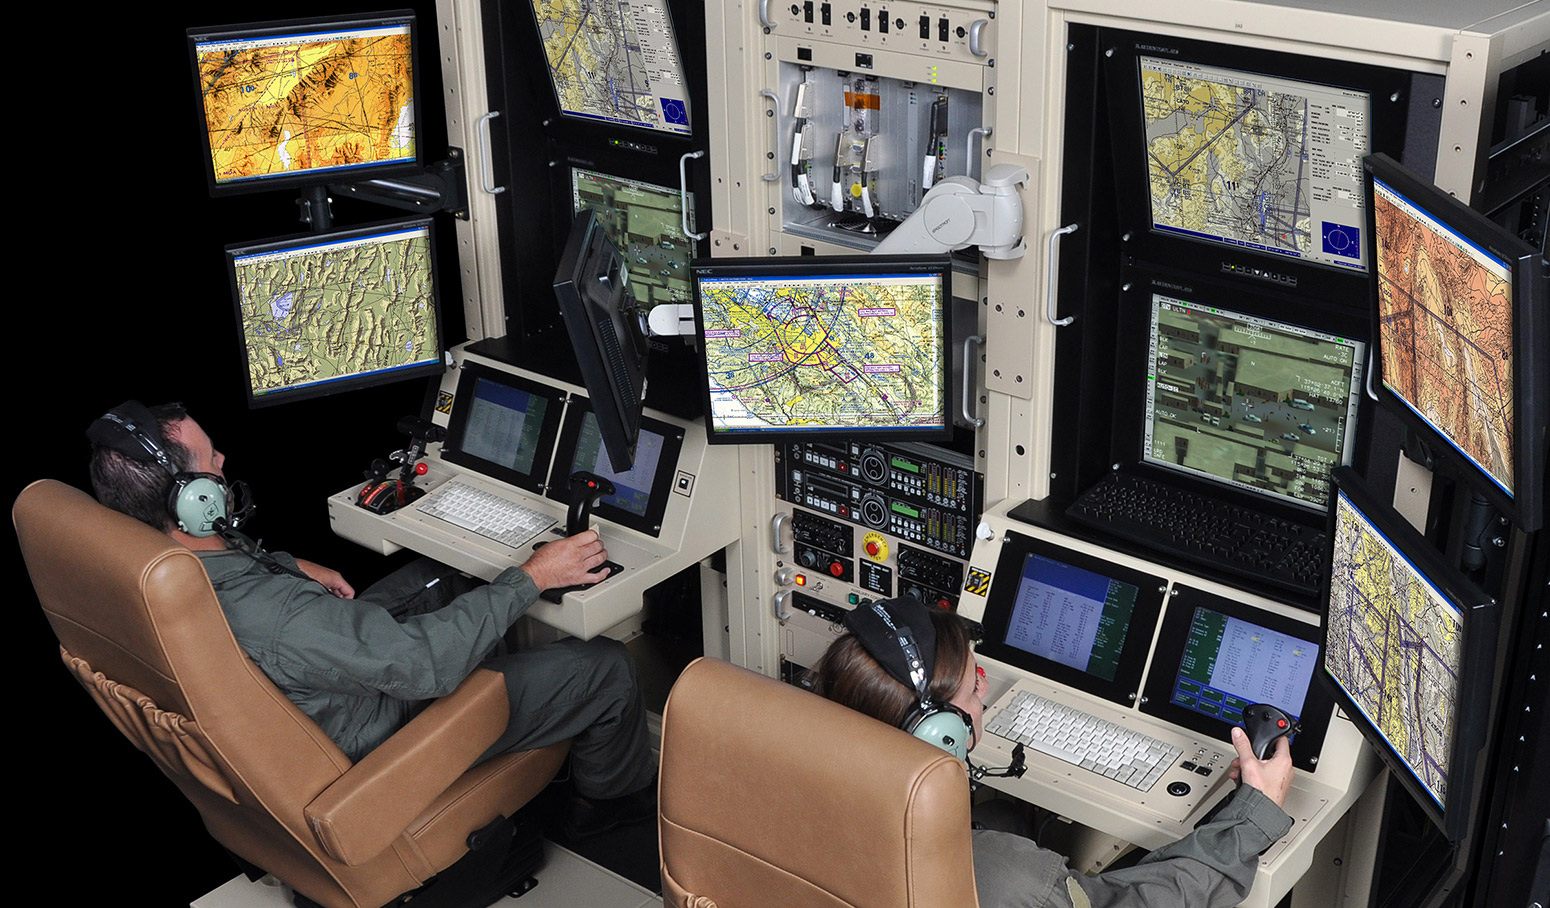
\includegraphics[scale=0.15]{uavpilotavoidbadweather}
	\end{center}
	\caption{Pilotaggio di un drone militare da remoto.\label{fig:uavpilotavoidbadweather}}
\end{figure}
%
Il volo autonomo è reso possibile tramite tecniche di intelligenza artificiale, utilizzando appositi sensori montati sul drone (come GPS o videocamere) per individuare ostacoli, conoscere la propria posizione e pianificare la rotta, spesso organizzata in waypoints. 
L'autonomia può essere completa, nel caso in cui tutte le decisioni sul movimento e le azioni sono elaborate dal computer di bordo, oppure parziale, in cui il computer di bordo interviene solo in particolari situazioni, ad esempio quando il drone perde la connessione con il pilota. \\

\subsection[Cenni storici]{Cenni storici}
Gli UAV sono nati in ambito puramente militare, per compiere missioni offensive o di ricognizione in cui non si poteva garantire l'incolumità del pilota; il loro sviluppo, portato avanti soprattutto dagli Stati Uniti, Israele e dal Regno Unito, ha proseguito di pari passo con la corsa agli armamenti durante le grandi guerre del 1900. \\
I primi tentativi di realizzare velivoli senza pilota risalgono al periodo della Prima Guerra Mondiale, con l'obiettivo di creare degli “aerei bomba” (\figurename\ \ref{fig:Kettering_Bug}), che in futuro si sarebbero evoluti negli attuali missili teleguidati. 
%
\begin{wrapfigure}{R}{0.5\textwidth}
	\begin{center}
		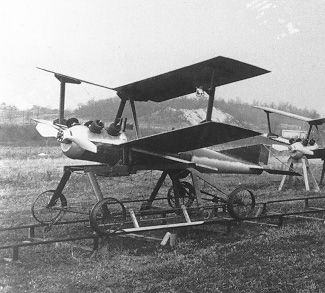
\includegraphics[scale=1.1]{KetteringBug}
	\end{center}
	\caption{Kettering Bug, uno dei primi prototipi di UAV militare, 1918.} \label{fig:Kettering_Bug}
\end{wrapfigure}
%
Furono perfezionati durante la Seconda Guerra Mondiale, e usati anche come bersagli mobili per addestrare gli addetti alla difesa contraerea, mentre conobbero un forte sviluppo durante i conflitti successivi agli anni '50, in cui vennero impiegati sia come armi offensive che come ricognitori per rimediare alle forti perdite di vite umane subite dall'aeronautica militare.  \\
I droni militari moderni sono nati a partire dagli anni '90: grazie al forte sviluppo dell'elettronica, la miniaturizzazione dei componenti e il conseguente abbattimento dei costi, l'interesse nei loro confronti è cresciuto sempre di più, fino a renderli una componente rilevante in molti eserciti contemporanei \cite{keane2013brief}.

\subsection[Ambiti d'uso]{Ambiti d'uso}
Come già accennato, in ambito militare i droni sono impiegati principalmente come ricognitori o bombardieri. 
Un nuovo metodo di impiego li vede coinvolti nel fornire supporto logistico alle truppe a terra, sia come trasporto attrezzatura sia come ponte radio per comunicazioni sicure tra squadre rimaste isolate. \\
L'impiego dei droni in campo civile invece è estremamente recente, e si studiano continuamente nuovi ambiti in cui poterli impiegare. 
Generalmente in questo campo si impiegano UAV di dimensioni ben più ridotte rispetto alle controparti militari, spesso veri e propri velivoli aerei. \\
Oltre allo scopo ricreativo e di fotografia aerea, sono stati impiegati con successo in agricoltura, per monitorare la salute del raccolto (la cosiddetta agricoltura di precisione) o irrigarlo, per ispezionare linee elettriche, condutture o edifici lesionati, nella sorveglianza domestica o di ampie aree geografiche, come supporto alle forze dell'ordine, nel monitoraggio della qualità ambientale dell'aria, come rilevatori di concentrazione di sostanze pericolose per l'uomo in seguito a disastri ambientali, nel supporto alle squadre di soccorso per individuare feriti o dispersi e per portare il prima possibile kit medici e defibrillatori agli operatori sanitari, come corrieri espressi per le spedizioni Amazon \cite{amazon}, contro il bracconaggio e per combattere incendi \cite{dronespeak}. 

\subsection[Tassonomia]{Tassonomia}
Non esiste un metodo unico per poter categorizzare efficacemente i droni, in quanto essi variano enormemente per caratteristiche tecniche e ambiti di utilizzo. Essi infatti possono essere suddivisi per:
\begin{itemize}
	\item Ambito:
		\begin{itemize}
			\item Militare: droni da combattimento, ricognitori, segnalatori di bersagli o esche anti-missile (decoys);
			\item Logistico: droni in grado di trasportare merci o attrezzature;
			\item Ricerca e sviluppo;
			\item Civile e commerciale: modellismo, riprese aeree, raccolta dati, supporto alle forze di soccorso, sorveglianza.
		\end{itemize}
	\item Altitudine e portata massimi \cite{uasglobal} :
		\begin{itemize}
			\item Portatili: fino a 600 m di altitudine e portata di 2 km; 
			\item Corto raggio: fino a 1500 m di altitudine e 10 km di portata;
			\item NATO e tattici: tra i 3000 e i 5000 m di altitudine e un range massimo di 160 km;
			\item Medio ed ampio raggio: fino a 9000 m e oltre i 200 km di portata. Oltre i 9000 m vengono definiti ad ampio raggio;
			\item Ipersonici:  fino a 15000 m, range superiore ai 200 km.
		\end{itemize}
	\item Dimensione e peso: qui la categorizzazione è meno precisa, in quanto ogni Paese definisce i propri standard:
		\begin{itemize}
			\item MAV (Micro Air Vehicle): droni che possono stare nel palmo di una mano. Recenti sviluppi hanno portato a modelli grandi pochi centimetri e del peso di alcuni grammi;
			\item SUAV (Small UAV): droni sufficientemente piccoli da essere trasportati da una persona e del peso non superiore ai 20-25 kg;
			\item HUAV (Heavy UAV):  in questa categoria rientrano tutti quei droni la cui struttura è comparabile, in dimensioni, a quella di un velivolo aereo. Hanno elevate capacità di trasporto e possono coprire elevate distanze prima di necessitare di rifornimento. Il loro uso è prevalentemente per scopi militari o di rilevamento.
		\end{itemize}
	\item Configurazione di volo: determina la struttura, la tipologia di motori e gli ambiti in cui può essere impiegato con maggior efficienza. Le principali versioni sono mostrate in \figurename\ \ref{fig:struttura}: 
		\begin{itemize}
			\item Multi-rotori: droni che impiegano più di due rotori per il volo. Hanno avuto ampia diffusione in ambito commerciale e modellistico grazie alla semplicità di costruzione, alla stabilità del volo e alla maggior capacità di carico. Le principali limitazioni sono bassa autonomia di volo e ridotta velocità;
			\item Ad ala fissa: sono equipaggiati con ali simili a quelle degli aerei, dispongono di buona autonomia ma non sono capaci di effettuare volo stazionario. Inoltre non sono generalmente in grado di decollare e atterrare in maniera autonoma, richiedendo sistemi simili a catapulte e paracadute;
			\item A rotore singolo: dispongono di un solo rotore, rendendoli concettualmente simili a un elicottero. Ciò li rende energeticamente molto più efficienti rispetto ai multi-rotore, a discapito di una maggiore complessità di costruzione e minore stabilità di volo;
			\item Ibridi: i più recenti, combinano la struttura ad ala fissa con uno o più rotori, posizionati in coda o verso il suolo, ottenendo i benefici di entrambe le configurazioni. 
		\end{itemize}
\end{itemize}
%
\begin{figure}
	\centering
	\begin{subfigure}[b]{0.4\textwidth}
		\centering
		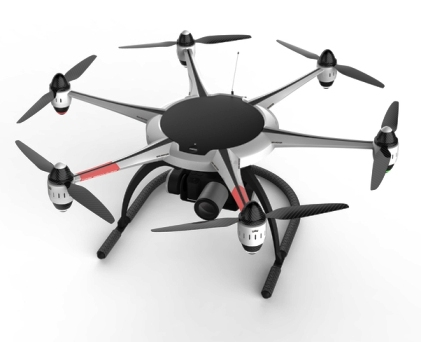
\includegraphics[scale= 1]{sixrotor}
		\caption{Multi-rotore}
		\label{fig:multirotor}
	\end{subfigure}
	%
	\begin{subfigure}[b]{0.4\textwidth}
		\centering
		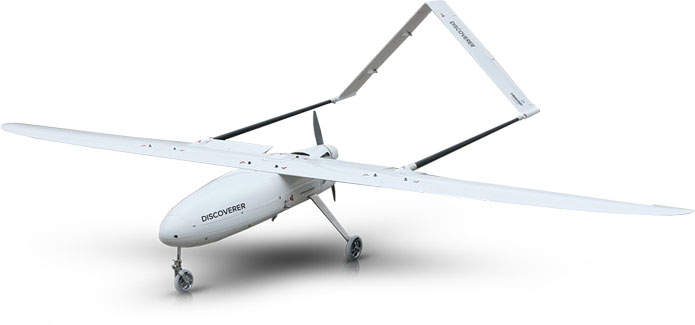
\includegraphics[scale= 0.2]{fixed}
		\caption{Ad ala fissa}
		\label{fig:fixed}
	\end{subfigure}
	%
	\begin{subfigure}[b]{0.4\textwidth}
		\centering
		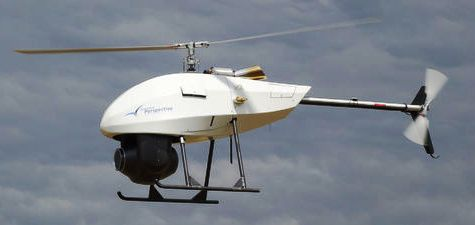
\includegraphics[scale= 1.5]{singlerotor}
		\caption{Singolo rotore}
		\label{fig:singlerotor}
	\end{subfigure}
	%
	\begin{subfigure}[b]{0.4\textwidth}
		\centering
		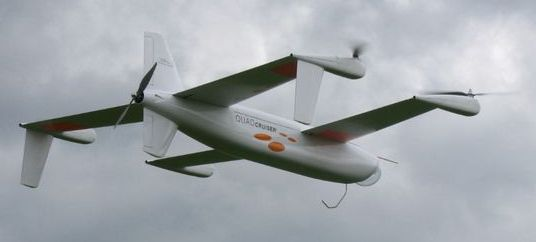
\includegraphics[scale = 0.39]{hybrid}
		\caption{Ibrido}
		\label{fig:hybrid}
	\end{subfigure}
	\caption{Principali configurazioni di volo dei droni}
	\label{fig:struttura}
\end{figure}
%
\subsection[Struttura]{Struttura}
La struttura di un drone, evidenziata in \figurename\ \ref{fig:uavstructure} è generalmente ricorrente, e può essere schematizzata nelle seguenti componenti \cite{Sahingoz2014}:

\begin{itemize}
	\item Fusoliera: l'assenza di equipaggio a bordo permette di poterla costruire con materiali più leggeri ed economici. Dimensione e forma variano grandemente in base alla funzionalità del drone e al peso che deve trasportare;
	\item Alimentazione: i droni di ridotta dimensione, come i MAV e gli SUAV, sono generalmente alimentati da batterie, mentre quelli più grandi richiedono i motori convenzionali di un aereo;
	\item Sensori: i sensori che il drone monta ne definiscono le funzionalità e le capacità di volo autonomo. Possono essere usati per raccogliere dati (sensori ambientali, fotocamere, videocamere), per la guida del drone da remoto, per evitare collisioni con ostacoli, per la navigazione autonoma (GPS, giroscopi, altimetri, accelerometri);
	\item Attuatori: sono i dispositivi, generalmente elettronici, che comandano i motori del drone e ne regolano l'assetto;
	\item Payload: è l'equipaggiamento trasportato dal drone, ed include sensori, trasmittenti, attrezzature, armi, etc. Generalmente il payload è contenuto in uno spazio interno apposito, per non influire sulle capacità aerodinamiche del mezzo;
	\item Computer di bordo e software: i droni sono dispositivi real-time, e sono equipaggiati con una o più unità di calcolo (microcontrollori, single-board computers, sistemi embedded, etc.)  per gestire il volo autonomo e i processi di decision-making. Le capacità di elaborazione degli UAV quindi crescono di pari passo con lo sviluppo e la miniaturizzazione dell'hardware;
	\item Sistemi di comunicazione: i sistemi di comunicazione del drone sono generalmente ad onde radio, e possono avvenire con l'operatore a terra in maniera diretta o indiretta (tramite un satellite o un altro velivolo), in base alla reciproca distanza. Il flusso di comunicazione è tipicamente composto in uplink dai comandi dell'operatore, e in downlink da segnali video, telemetria o rilevazioni dei sensori. Molti  MAV e SUAV comunicano via Wi-Fi, rendendo possibile pilotarli tramite smartphone o tablet.  
\end{itemize}
%
\begin{figure}
	\begin{center}
		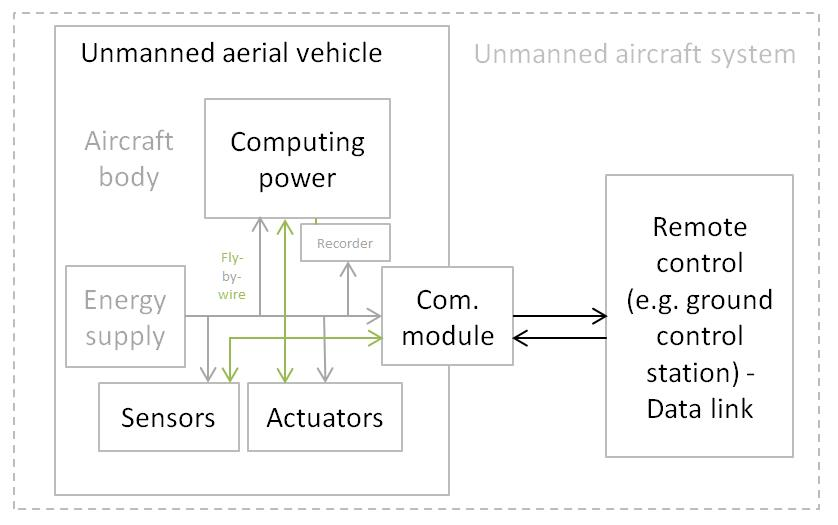
\includegraphics[scale=0.5]{uavstructure}
	\end{center}
	\caption{Schema a blocchi dei principali componenti di un drone} \label{fig:uavstructure}
\end{figure}
%
\subsection[Autonomia di volo]{Autonomia di volo} \label{sect:autonomia}
Una delle attuali sfide nel mondo degli Small UAV è l'incremento del loro tempo di volo, che generalmente non supera i 10-20 minuti prima di dover effettuare la ricarica della batteria. \\
Forza del vento, tipologia dei sensori installati, peso del drone e frequenza di movimento sono i principali fattori che incidono sul consumo della batteria. 
È possibile caricare il drone con più batterie in parallelo, ma più batterie equivalgono a maggior peso da sollevare e a un conseguente maggior consumo di energia da parte dei motori, rendendo quindi risibile il contributo di più batterie alla durata di volo.\\
Negli ultimi anni è stata esplorata la strada dei pannelli solari come fonte energetica ausiliaria per incrementare l'autonomia di volo (\figurename\ \ref{fig:solar}). 
%
\begin{figure}
	\centering
	\begin{subfigure}[b]{0.4\textwidth}
		\centering
		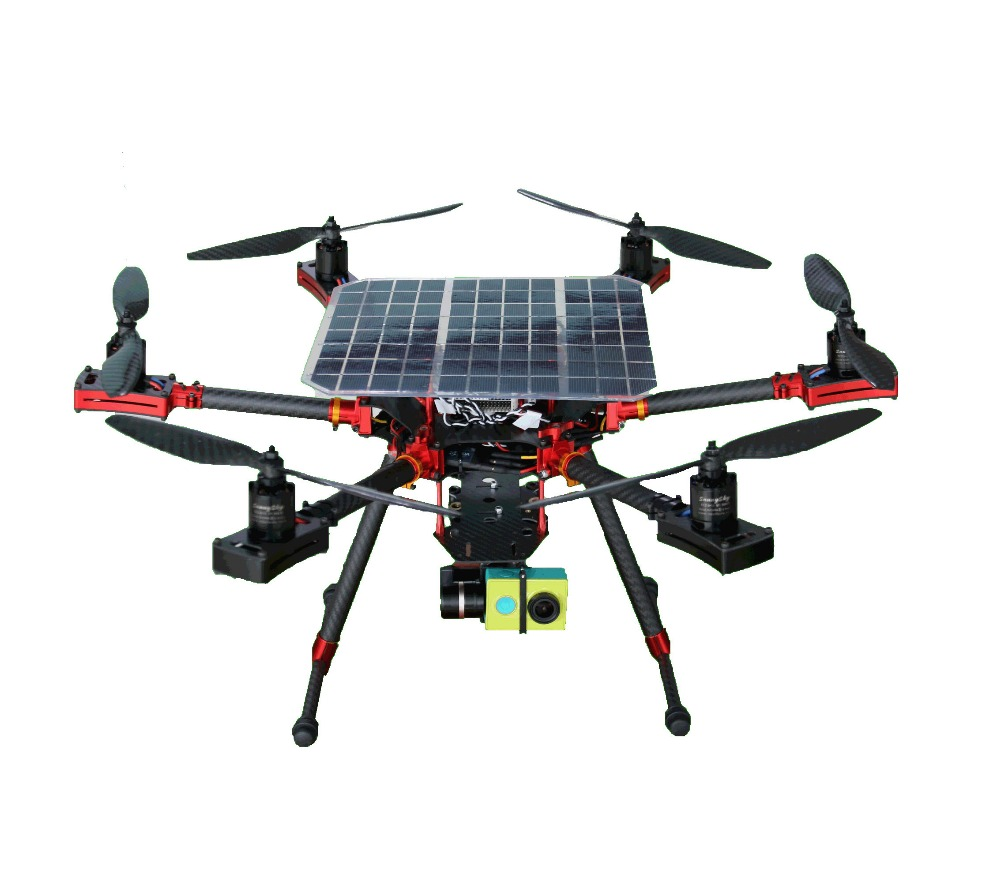
\includegraphics[scale= 0.15]{solarquad}
		\caption{Multi-rotore solare}
		\label{fig:solarquad}
	\end{subfigure}
	%
	\begin{subfigure}[b]{0.4\textwidth}
		\centering
		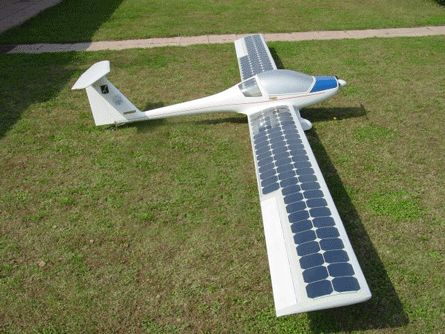
\includegraphics[scale= 0.4]{solarfixed}
		\caption{Ad ala fissa solare}
		\label{fig:solarfixed}
	\end{subfigure}
	\caption{Prototipi di droni ad energia solare}
	\label{fig:solar}
\end{figure}
%
I risultati migliori, seppur ancora lontani dall'autonomia energetica, sono stati ottenuti sui droni ad ala fissa \cite{newatlas} ricoprendo le ali di pannelli, mentre sui quadrirotori l'ingombro dell'attrezzatura aggiuntiva causava un effetto vela che riduceva la stabilità in volo \cite{diydrones}.\\ Se in campo commerciale ed amatoriale i risultati sono stati poco incoraggianti, non è andata così nel campo dei grandi velivoli: seppur guidato da un pilota, il progetto Solar Impulse 2, un aereo completamente alimentato dall'energia solare, ha completato il giro del mondo nell'estate del 2016 \cite{theguardian}, mentre Facebook sta attivamente testando l'uso di droni solari per fornire connettività a internet ai Paesi del Terzo Mondo con il progetto Aquila \cite{fbaquila}.\\

\section[Reti ad-hoc]{Reti ad-hoc}
Una rete Ad-hoc è una tipologia di WLAN decentralizzata in cui è assente la tradizionale infrastruttura delle reti managed (AP, router, switch, etc.), in quanto sono gli stessi nodi a occuparsene, agendo come routers. \\
La rete ad-hoc consiste in un gruppo di client mobili che formano spontaneamente una rete temporanea, dinamica e auto-configurante (ad esempio, per comunicare o condividere dati). 
Ciascun nodo potrà comunicare direttamente con tutti quelli entro il suo range trasmissivo, e tramite multi-hop con quelli al di fuori di esso (\figurename\ \ref{fig:manet}). \\
%
\begin{figure}
	\begin{center}
		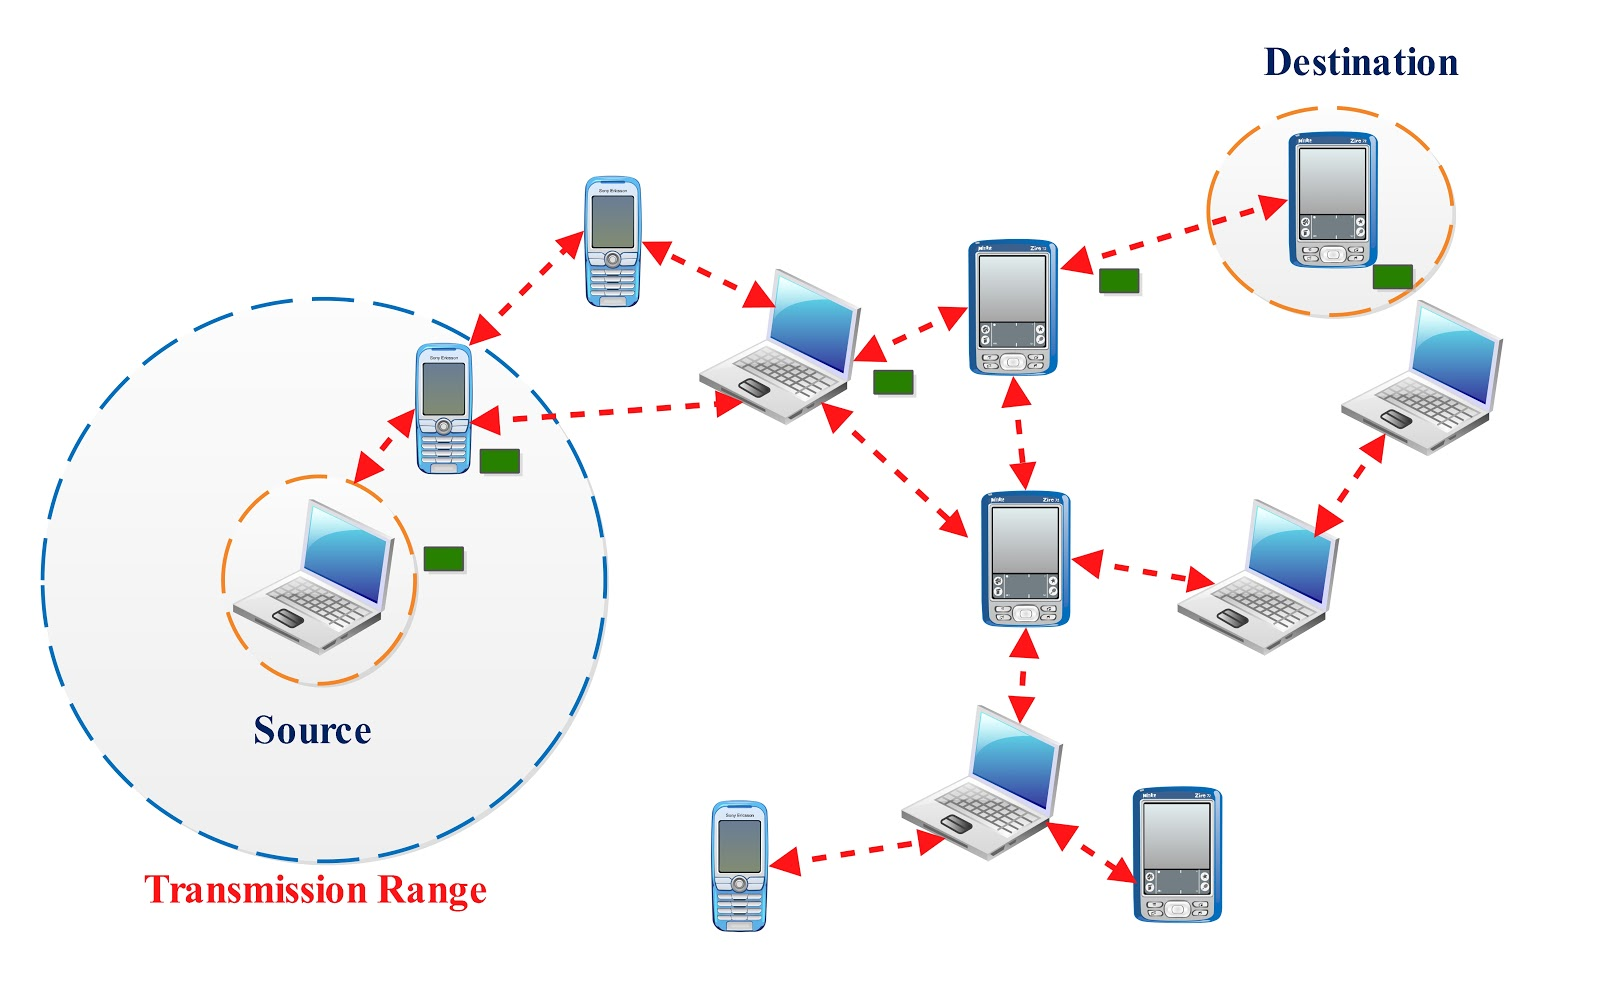
\includegraphics[scale=0.2]{manet}
	\end{center}
	\caption{Esempio di comunicazione multi-hop in rete ad-hoc.} \label{fig:manet}
\end{figure}
%
Poiché i client sono liberi di muoversi, la topologia di queste reti tende a cambiare velocemente e in maniera non prevedibile: possono verificarsi variazioni di routes, partizionamento del grafo di rete, fluttuazioni nella capacità dei link, con conseguente perdita di pacchetti, perciò i protocolli di rete devono avere un alto grado di adattabilità e reattività, per  monitorare lo stato dei link e regolare i flussi di traffico di conseguenza.
L'assenza di infrastruttura di routing dedicata richiede che il network management sia distribuito tra tutti i nodi, per esempio tramite flussi di traffico di controllo, aggiungendo un ulteriore livello di complessità. \\
Le reti ad-hoc sono tipicamente impiegate in quelle situazioni in cui l'infrastruttura di rete è assente, inadatta o compromessa: alcuni casi d'uso possono essere la condivisione di dati in un meeting, comunicazioni militari, networking, servizi veicolari (trasmissione di news, intensità del traffico, musica, etc.), gaming, o l'instaurazione di sistemi di comunicazione per le squadre di soccorso in seguito a calamità naturali \cite{7402025}. \\
I principali vantaggi delle reti ad-hoc sono la capacità di auto-configurazione dei nodi, richiedendo un intervento minimo dell'utente, la velocità di deployment, il self-healing, ovvero la capacità della rete di riconfigurarsi autonomamente in seguito a un cambio della sua topologia, la scalabilità e i costi ridotti dovuti dall'assenza dell'infrastruttura.\\
I principali svantaggi di questo tipo di architettura sono la necessità di un elevato grado di adattabilità dei protocolli, a causa dei frequenti cambi di topologia nella rete, l'eterogeneità dei client, in quanto le diverse capacità di trasmissione, ricezione e calcolo dei dispositivi possono causare link asimmetrici, la dipendenza dei client dalla batteria del loro device, la cui durata viene ulteriormente ridotta dalle funzionalità di routing, e la vulnerabilità ad attacchi, a causa dell'assenza di una struttura centrale di autenticazione. \cite{jayakumar2007ad}
\\
In particolare, anche il power management dei nodi può influenzare la topologia della rete: un client può scegliere se aumentare la potenza di trasmissione (e il suo range, di conseguenza) per spedire direttamente un pacchetto al destinatario, oppure ridurla e fare affidamento sulla consegna multi-hop.\\
Questa scelta porta alla creazione e cancellazione di path, e alla modifica della topologia. 
Entrambi gli approcci hanno degli svantaggi: trasmettere a maggior potenza riduce il ritardo nella consegna dei messaggi, ma aumenta il consumo della batteria e riduce il throughput della rete, in quanto all'aumento del range corrisponde un aumento nella zona di interferenza, e tutti i nodi interni a questa area dovranno restare silenti fino al termine della trasmissione; la trasmissione a bassa potenza invece riduce il consumo della batteria e aumenta la capacità della rete, ma incrementa il ritardo medio dei pacchetti perché devono passare per più hop prima di giungere a destinazione. \\
Generalmente un compromesso viene raggiunto regolando dinamicamente la potenza trasmissiva e creando una condivisione di informazioni tra i protocolli di rete e i layer sottostanti. \cite{879383}

\subsection[Protocolli di routing]{Protocolli di routing}
I protocolli di routing vengono impiegati per determinare i path più efficienti (in termini di costi, ritardo, consumo energetico, etc.) attraverso i nodi della rete, che permettano ai messaggi di raggiungere la propria destinazione. \\
Il routing nelle reti ad-hoc deve tenere conto della mobilità dei nodi e delle loro limitate capacità energetiche e di calcolo. 
Questi due aspetti hanno soluzioni conflittuali, in quanto il primo richiede frequenti scambi di informazioni e aggiornamenti delle tabelle di routing, mentre il secondo li dovrebbe minimizzare, riducendo le trasmissioni e mantenendo tabelle di piccole dimensioni. \\
Si possono identificare due principali famiglie di protocolli di routing per le reti ad-hoc: protocolli proattivi e on demand.\\
I protocolli proattivi, di cui fanno parte le famiglie Link State e Distance Vector, effettuano un monitoraggio costante della rete e ne mantengono uno “stato” tramite le tabelle di routing. 
Al verificarsi di un cambiamento nella topologia, inviano messaggi (control traffic) agli altri nodi con le correzioni da apportare alle tabelle.\\ Permettono un rapido inoltro dei pacchetti grazie alle informazioni sempre aggiornate, ma la presenza costante di traffico di controllo introduce un overhead che cresce con la frequenza dei cambi di topologia, e in reti molto dinamiche può portare all'impossibilità di tenere traccia di tutti gli aggiornamenti delle stesse. Esempi di protocolli proattivi sono DSDV (Highly Dynamic Destination-Sequenced Distance Vector routing protocol), HSLS (Hazy Sighted Link State routing protocol), OLSR (Optimized Link State Routing Protocol) e STAR (Source Tree Adaptive routing protocol).\\
I protocolli on demand (o reattivi), invece, usano un approccio “lazy”, cioè non si preoccupano di mantenere una tabella di path aggiornati, ma richiedono il path di destinazione tramite flooding solo all'ultimo momento, quando sono presenti pacchetti che necessitano di essere instradati.
Questa tecnica permette una maggior scalabilità e non necessita di traffico di controllo, ma introduce un costante ritardo, detto setup delay, sul primo pacchetto che deve essere spedito a una nuova destinazione (che può diventare gravoso nel caso di traffico intermittente), e rende la rete vulnerabile ad attacchi basati sul flooding. Protocolli reattivi sono AODV (Ad hoc On Demand Distance Vector routing protocol) e DSR (Dynamic Source Routing) \cite{879383}. \\
Vi è poi una terza categoria, i protocolli ibridi, che cercano di combinare i vantaggi delle due famiglie, facendo routing proattivo per un ristretto gruppo di nodi (i nodi inizialid ella rete, o quelli considerati più “vicini”) e routing on demand su tutti gli altri. Un esempio è il protocollo ZRP (Zone Routing Protocol).\\

\subsection[Reti Infrastructure VS reti Ad-hoc]{Reti Ad-hoc VS Infrastructure}
Lo standard IEEE 802.11 per le Wireless Local Area Network (WLAN) prevede due principali modalità di funzionamento delle reti Wi-Fi: modalità infrastruttura (o managed) e modalità ad-hoc (\figurename\ \ref{fig:adhoc}). \\
%
\begin{figure}
	\begin{center}
		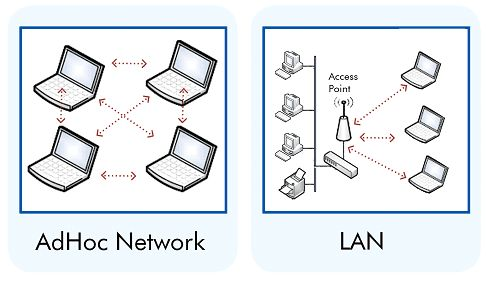
\includegraphics[scale=0.7]{adhoc}
	\end{center}
	\caption{Rete Infrastructure (a sinistra) e rete Ad-hoc (a destra).} \label{fig:adhoc}
\end{figure}
%
La modalità infrastruttura, generalmente più diffusa, prevede la presenza di base stations (Wireless Access Points, o APs) cui i client devono connettersi per poter comunicare tra loro. La comunicazione diretta client-client quindi non è ammessa, ma deve essere veicolata passando per l'AP. \\
Le base station, che svolgono una funzionalità di hub, a loro volta sono connesse, generalmente via cavo, all'infrastruttura centrale della rete e a un router. Esse sono generalmente fisse e forniscono connettività ai nodi client entro il proprio range.\\
Le reti infrastructure, come dice il nome, si appoggiano a una infrastruttura di rete, perciò sono generalmente pensate con un concetto di permanenza della stessa. 
La loro installazione e progettazione richiede costi in termini di denaro e tempo, mentre le reti ad-hoc non richiedono dispositivi aggiuntivi e si auto-configurano automaticamente in tempi rapidi. 
Le antenne degli AP sono generalmente più potenti di quelle equipaggiate da laptop o smartphone, permettendo quindi di comunicare a range superiori.  
Le reti ad-hoc in generale impongono ai client un maggior consumo di risorse di sistema per far fronte alla mobilità dei nodi e al conseguente cambio della topologia, mentre nelle reti managed gli APs sono generalmente fissi. Questo fattore risulta critico se si considera che i tipici client delle reti ad-hoc sono dotati di batteria, e di conseguenza in questa tipologia di rete la loro autonomia sarà minore.
Infine, le reti ad-hoc tendono a non scalare bene con il numero di client, a causa della maggior interferenza causata dalle numerose connessioni dirette tra client.

\section[Reti FANET]{Reti FANET}
Generalmente le reti ad-hoc vengono categorizzate in base alla tipologia dei client che le compongono. Le principali, schematizzate in \tablename\ \ref{tab:adhoc}  sono: MANETs (Mobile), VANETs (Vehicular), SPANs (Smartphone) e FANET (Flying). \\
Le reti FANET sono reti ad-hoc, ancora in fase sperimentale, tra droni equipaggiati con antenne radio, e possono essere viste come un sottoinsieme delle VANET (\figurename\ \ref{fig:fanet}), pur differendone sostanzialmente in termini di capacità, requisiti e problematiche. 
%
\begin{figure}
	\begin{center}
		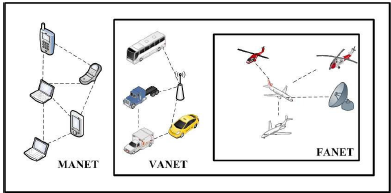
\includegraphics[scale=0.8]{fanet}
	\end{center}
	\caption{Tipologie di reti ad-hoc} \label{fig:fanet}
\end{figure}
%
Tali reti possono essere impiegate sia per lo scambio di informazioni tra droni, per esempio per coordinarsi nel volo autonomo in “stormo”, sia come relay per mettere in comunicazione client a terra. \\
Attualmente le FANET impiegano soprattutto gli heavy UAVs, per sfruttarne la maggior potenza di calcolo e trasmissione, oltre che la maggior autonomia di volo, ma grazie alla progressiva riduzione dei costi di produzione si sta sperimentando l'uso di molteplici Small UAVs. \\
Anche se il singolo SUAV ha capacità limitate, l'impiego di una squadra di droni  porta i seguenti vantaggi:
\begin{itemize}
	\item Aumenta la ridondanza, in quanto se un drone diventa offline i restanti possono riorganizzarsi e mantenere funzionante la rete, anche se a performance ridotte;
	\item Più droni possono parallelizzare il lavoro e ridurre i tempi della missione;
	\item Riduzione dei costi, impiegando più SUAVs economici rispetto un singolo e costoso HUAV;
	\item Aumenta la scalabilità, in quanto per coprire un'area di operazione maggiore basta aggiungere droni;
	\item Possono cooperare e sfruttare le reciproche funzionalità, utile soprattutto se equipaggiati in maniera differente gli uni dagli altri.
\end{itemize}
In una FANET si possono distinguere due modelli di comunicazione, che necessitano di protocolli differenti:
\begin{itemize}
	\item Comunicazione drone-drone: la comunicazione può essere diretta o multihop, e generalmente riguarda il coordinamento di volo e la cooperazione nel compiere un dato task;
	\item Comunicazione drone-infrastruttura: la comunicazione avviene tra il drone e una ground station (o un satellite) e generalmente consiste nel fornire i dati rilevati dai sensori del drone.
\end{itemize}
Come già accennato, le reti FANET rappresentano ancora un nuovo campo per la ricerca, e prima che possano raggiungere il loro potenziale devono essere risolte ancora molte problematiche. \\
In base alla tipologia di drone impiegato ci si può aspettare differenti gradi di mobilità dei nodi, dal volo stazionario del piccolo quadri-rotore all'alta velocità degli HUAVs, e quindi una diversa frequenza di variazione della topologia. 
Gli stessi droni possono viaggiare a velocità diversa, guastarsi o allontanarsi per ricaricarsi, creando partizionamenti e continue riorganizzazioni della rete. \\
Il consumo energetico è un altro fattore chiave nelle FANET: mentre nelle MANET i devices hanno  autonomie di svariate ore e nelle VANET i veicoli ricaricano la batteria grazie al movimento del mezzo, nelle FANET i piccoli droni possono restare in volo solo poche decine di minuti, perciò i protocolli di queste ultime devono minimizzare il consumo energetico, favorendo per esempio trasmissioni a bassa potenza e routing multihop. 
La presenza di molteplici droni aggiunge un ulteriore complessità, in quanto occorrono protocolli di coordinazione, organizzazione e path-planning.
Quest'ultimo consente ai droni di modificare il proprio percorso in reazione a cambiamenti dinamici, come la presenza di ostacoli. \\
Queste problematiche dimostrano che affinché le FANET possano essere impiegate efficacemente sono necessari nuovi  protocolli di comunicazione, coordinamento e cooperazione tra droni. \\
Nonostante le somiglianze tra le tipologie di rete, i protocolli usati nelle reti MANET e VANET generalmente non sono utilizzabili nelle FANET o hanno scarse performance, perciò occorre definire nuovi algoritmi di routing dedicati e prevedere modifiche ai layers MAC e network \cite{7317490}.

\begin{table}[]
	\small
	\centering
	\begin{tabular}{|p{2.2cm}|p{3cm}|p{3cm}|p{3cm}|}
		\hline
		& MANET                                                                                                         & VANET                                                                                                                                                                                                 & FANET                                                                                                                                     \\ \hline
		Tipo di nodo       & Mobile devices (tablet, laptop, smartphone, etc.)                                                             & Veicoli                                                                                                                                                                                               & Droni                                                                                                                                     \\ \hline
		Descrizione        & Dispositivi mobile in range tra loro si interconnettono in una rete ad-hoc, senza necessità di infrastrutture & Veicoli connessi tra di loro. La comunicazione avviene tra veicoli e tra veicoli e nodi di supporto (Roadside Units) disposti lungo la strada              & I droni costruiscono una rete ad-hoc fra di loro e i nodi a terra                                                                         \\ \hline
		Mobilità           & Lenta, generalmente al di sotto dei 2 m/s. Il pattern di movimento è tipicamente casuale                      & Alta velocità, in base alla tipologia di strada (urbana o aoutostradale). Il pattern di movimento è generalmente prevedibile in quanto vincolato dalla struttura della strada e dalle norme stradali. & Molto variabile, da stazionario a oltre i 100 m/s, a seconda della tipologia di drone. Il movimento può avvenire in due o tre dimensioni. \\ \hline
		Topologia          & Casuale, ad-hoc                                                                                               & A stella tra veicoli e infrastruttura stradale, ad-hoc tra i veicoli                                                                                                                                  & A stella tra droni e ground control, ad-hoc o a mesh tra droni                                                                            \\ \hline
		Dinamicità         & I nodi entrano ed escono dalla rete in maniera imprevedibile, frequenti partizionamenti                       & Maggior dinamicità rispetto la MANET, a causa della maggior velocità dei nodi e delle interferenze del traffico                                                                                       & Variabile, in base alla velocità relativa dei droni                                                                                       \\ \hline
		Vincoli energetici & Nodi con batteria, autonomia di alcune ore                                                                    & Batteria dei veicoli si ricarica con il movimento                                                                                                                                                     & Durata della batteria proporzionale alla dimensione dello UAV                                                                             \\ \hline
		Ambiti d'uso       & Distribuzione dell'informazione, hot spot internet, networking                                                & Informazioni di traffico, servizi location based, avvisi di emergenza                                                                                                                                 & Sorveglianza, salvataggio, distribuzione, monitoraggio                                                                                    \\ \hline
	\end{tabular}
	\caption{Confronto tra le diverse tipologie di reti ad-hoc} \label{tab:adhoc}
\end{table}

\subsection[Routing nelle FANET]{Routing nelle FANET}
Attualmente l'implementazione di algoritmi di routing per FANET ha seguito due strade: creazione di protocolli ad-hoc e modifiche di algoritmi preesistenti per MANET e VANET. \\
Si possono distinguere quattro tipologie di protocolli:
\begin{itemize}
	\item Statici: le tabelle di routing vengono pre-calcolate e caricate sul drone, per poi non essere più modificate fino al termine della missione. Questa forte limitazione può essere tollerata solo nei casi in cui la topologia della rete rimane fissa nel tempo. Esempi di questa famiglia di protocolli sono LCAD ( Load Carry and Deliver Routing) e il Multi-Level Hierarchical Routing;
	\item Proattivi: sono gli algoritmi table-driven per le reti ad-hoc precedentemente descritti. Impiegati nelle FANET garantiscono velocità nel routing, ma la loro necessità di scambiare traffico di controllo aggrava la già ridotta disponibilità di bandwith. Inoltre non sono adatti per reti di grandi dimensioni e in cui i nodi si muovono molto velocemente, poiché hanno tempi di reazione ai cambiamenti di topologia molto lunghi.
	\item Reattivi: precedentemente descritti come algoritmi on-demand, garantiscono un uso efficiente della banda in quanto non necessitano di traffico di controllo e scambi periodici di messaggi, ma introducono forti delay a causa della tipologia di traffico tipicamente intermittente delle FANET. 
	\item Ibridi: cercano di unire i vantaggi dei protocolli proattivi e reattivi, riducendo la latenza iniziale e l'overhead dei messaggi di controllo, e sono efficaci anche in reti di grandi dimensioni. 
\end{itemize}





% Uncomment this line, when you have siunitx package loaded.
%The SI Units for dynamic viscosity is \si{\newton\second\per\metre\squared}.


\chapter{My third chapter}

% **************************** Define Graphics Path **************************
\ifpdf
    \graphicspath{{Chapter3/Figs/Raster/}{Chapter3/Figs/PDF/}{Chapter3/Figs/}}
\else
    \graphicspath{{Chapter3/Figs/Vector/}{Chapter3/Figs/}}
\fi

\begin{table}
\caption{A badly formatted table}
\centering
\label{table:bad_table}
\begin{tabular}{|l|c|c|c|c|}
\hline 
& \multicolumn{2}{c}{Species I} & \multicolumn{2}{c|}{Species II} \\ 
\hline
Dental measurement  & mean & SD  & mean & SD  \\ \hline 
\hline
I1MD & 6.23 & 0.91 & 5.2  & 0.7  \\
\hline 
I1LL & 7.48 & 0.56 & 8.7  & 0.71 \\
\hline 
I2MD & 3.99 & 0.63 & 4.22 & 0.54 \\
\hline 
I2LL & 6.81 & 0.02 & 6.66 & 0.01 \\
\hline 
CMD & 13.47 & 0.09 & 10.55 & 0.05 \\
\hline 
CBL & 11.88 & 0.05 & 13.11 & 0.04\\ 
\hline 
\end{tabular}
\end{table}

\begin{table}
\caption{A nice looking table}
\centering
\label{table:nice_table}
\begin{tabular}{l c c c c}
\hline 
\multirow{2}{*}{Dental measurement} & \multicolumn{2}{c}{Species I} & \multicolumn{2}{c}{Species II} \\ 
\cline{2-5}
  & mean & SD  & mean & SD  \\ 
\hline
I1MD & 6.23 & 0.91 & 5.2  & 0.7  \\

I1LL & 7.48 & 0.56 & 8.7  & 0.71 \\

I2MD & 3.99 & 0.63 & 4.22 & 0.54 \\

I2LL & 6.81 & 0.02 & 6.66 & 0.01 \\

CMD & 13.47 & 0.09 & 10.55 & 0.05 \\

CBL & 11.88 & 0.05 & 13.11 & 0.04\\ 
\hline 
\end{tabular}
\end{table}


\begin{table}
\caption{Even better looking table using booktabs}
\centering
\label{table:good_table}
\begin{tabular}{l c c c c}
\toprule
\multirow{2}{*}{Dental measurement} & \multicolumn{2}{c}{Species I} & \multicolumn{2}{c}{Species II} \\ 
\cmidrule{2-5}
  & mean & SD  & mean & SD  \\ 
\midrule
I1MD & 6.23 & 0.91 & 5.2  & 0.7  \\

I1LL & 7.48 & 0.56 & 8.7  & 0.71 \\

I2MD & 3.99 & 0.63 & 4.22 & 0.54 \\

I2LL & 6.81 & 0.02 & 6.66 & 0.01 \\

CMD & 13.47 & 0.09 & 10.55 & 0.05 \\

CBL & 11.88 & 0.05 & 13.11 & 0.04\\ 
\bottomrule
\end{tabular}
\end{table}

 \chapter{Stato dell'arte e strumenti}

% **************************** Define Graphics Path **************************
\ifpdf
    \graphicspath{{Chapter4/Figs/Raster/}{Chapter4/Figs/PDF/}{Chapter4/Figs/}}
\else
    \graphicspath{{Chapter4/Figs/Vector/}{Chapter4/Figs/}}
\fi

\section{Stato dell'arte}


 \chapter{Il modello I-DARNC} \label{chap:modello}
 In questo capitolo presenteremo il modello di programmazione lineare intera I-DARNC (Interference-aware  Drone Ad-hoc Relay Network Configuration problem) per il posizionamento minimo e ottimale di un gruppo di droni per mettere in comunicazione gruppi di utenti isolati tra loro, soddisfacendo le loro richieste di traffico. Verranno poi presentate le formulazioni alternative più rilevanti incontrate durante il suo sviluppo.\\

% **************************** Define Graphics Path **************************
\ifpdf
    \graphicspath{{Chapter5/Figs/Raster/}{Chapter5/Figs/PDF/}{Chapter5/Figs/}}
\else
    \graphicspath{{Chapter5/Figs/Vector/}{Chapter5/Figs/}}
\fi

\section{Formulazione del modello}

\begin{figure}
	
		\begin{equation*} \label{eq:fo}
		\begin{array}{rrclcl}
		\displaystyle \min & \displaystyle \sum_{v \in P} y_{v} \phantom{XXXXXXXXXXXXXXXXXXXXXXXXXXXXXXXXX}\\
		\textrm{s.t.}\\
		\end{array}
		\end{equation*}
		
		% 1
		\begin{equation} \label{eq:balance}
		\begin{array}{rrclcl}
		&\displaystyle \sum_{\substack{i \in V \cup P:\\ d_{iv} \le R}} f^{sd}_{iv} - \displaystyle \sum_{\substack{j \in V \cup P:\\ d_{vj} \le R}} f^{sd}_{vj} & = & B^{sd}_{v} && \forall \; v \in V \cup P, \; (s,d) \in K \\
		\end{array}
		\end{equation}
		
		% 2
		% % %	\begin{subequations} \label{eq:activeY}
		% % %				\begin{equation} \label{eq:2a}
		% % %				\begin{array}{rrclcl}
		% % %					& f^{sd}_{ij} & \leq & T^{sd} \, y_{i} && \forall \; i \in P, \; j \in V \cup P, \; i \neq j, \; (s,d) \in K\\
		% % %				\end{array}
		% % %				\end{equation}
		% % %				
		% % %				\begin{equation} \label{eq:2b}
		% % %				\begin{array}{rrclcl}
		% % %					& f^{sd}_{ij} & \leq & T^{sd} \, y_{j} && \forall \; i \in V \cup P, \; j \in P, \; i \neq j, \; (s,d) \in K\\
		% % %				\end{array}
		% % %				\end{equation}
		% % %	\end{subequations}
		
		%	% 3
		%	\begin{subequations} \label{eq:3}
		%		\begin{equation} \label{eq:3a}
		%			\begin{array}{rrclcl}
		%				& x_{ij} & \leq & y_{j} && \forall i \in V', \forall j \in P, i \neq j\\
		%			\end{array}
		%		\end{equation}
		%		
		%		\begin{equation} \label{eq:3b}
		%			\begin{array}{rrclcl}
		%				& x_{ji} & \leq & y_{j} && \forall i \in V', \forall j \in P, i \neq j\\
		%			\end{array}
		%		\end{equation}
		%	\end{subequations}
		
		%	% 4
		%	\begin{equation} \label{eq:4}
		%		\begin{array}{rrclcl}
		%			& \displaystyle \sum_{i \in P} y_{i} & \leq & N_{UAV}\\
		%		\end{array}
		%	\end{equation}
		
		% 11
		%	\begin{subequations} \label{eq:11}
		\begin{equation} \label{eq:capTX}
		\begin{array}{rrclcl}
		& \displaystyle \sum_{j \in V \cup P} \displaystyle \sum_{(s,d) \in K} f^{sd}_{ij} (1 + A_{ij}) & \leq & U^{TX} y_{i} && \forall \; i \in P \\
		\end{array}
		\end{equation}
		
		%		\begin{equation} \label{eq:11b}
		%			\begin{array}{rrclcl}
		%				& \displaystyle \sum_{j \in P} \displaystyle \sum_{k \in K} f_{ijk} & \leq & U_{TX} && \forall i \in V \\
		%			\end{array}
		%		\end{equation}
		%	\end{subequations}		
		
		% 5
		%	\begin{subequations} \label{eq:5}
		\begin{equation} \label{eq:capRX}
		\begin{array}{rrclcl}
		&\displaystyle \sum_{j \in V \cup P} \displaystyle \sum_{(s,d) \in K} f^{sd}_{ji} & \leq & U^{RX} ( y_{i} - s_{i} ) && \forall \; i \in P\\
		\end{array}
		\end{equation}
		%		
		%		\begin{equation} \label{eq:5b}
		%			\begin{array}{rrclcl}		
		%				&\displaystyle \sum_{j \in P} \displaystyle \sum_{k \in K} f_{jik} & \leq & U_{RX} - s_{i} && \forall i \in V\\
		%			\end{array}
		%		\end{equation}
		%	\end{subequations}
		% 7
		%Let $ D_{i}^{\epsilon} = \{ j \in V : d(i,j) \leq R_{\epsilon} \}, $ where d(i,j) = euclidean distance between nodes i and j:  \\
		%	\begin{subequations} \label{eq:7}
		%		\begin{equation} \label{eq:7a}
		%			\begin{array}{rrclcl}
		%				&\displaystyle \sum_{j \in P : d(i,j) \leq R_{\epsilon}} y_{j} & \leq & M ( z_{i} + 1 - y_{i} ) && \forall i \in P : |D_{i}^{\epsilon}| = 0 \\ 
		%			\end{array}
		%		\end{equation}
		%		
		%		\begin{equation} \label{eq:7b}
		%			\begin{array}{rrclcl}
		%				&\displaystyle \sum_{j \in P : d(i,j) \leq R_{\epsilon}} y_{j} & \leq & M z_{i} && \forall i \in V : |D_{i}^{\epsilon}| = 0 \\ 
		%			\end{array}
		%		\end{equation}
		%		
		%		\begin{equation} \label{eq:7c}
		%			\begin{array}{rrclcl}
		%				&z_{i} & \geq & y_{i} && \forall i \in P : |D_{i}^{\epsilon}| > 0\\
		%			\end{array}
		%		\end{equation}
		%	\end{subequations}
		
		
		
		\begin{equation} \label{eq:set.z}
		\begin{array}{rrclcl}
		& z_{i} & \geq & y_{j} && \forall \; i , j \in P, \; i \neq j : \; d_{ij} \le R_{\epsilon} 
		\end{array}
		\end{equation}
		
		
		% 9
		%	\begin{subequations} \label{eq:9}
		\begin{equation} \label{eq:setSub}
		\begin{array}{rrclcl}
		& \displaystyle \sum_{\substack{j \in P :\\ R_{\epsilon} < d(i,j) \le R }} A_{ji} y_{j} + \displaystyle \sum_{\substack{j \in V :\\ d(i,j) \le R }} A_{ji} & \leq & S_{\max} + (M_i - S_{\max}) o_i %(o_{i} + 1 - y_{i}) 
		&& \forall \; i \in P\\
		\end{array}
		\end{equation}
		
		%		\begin{equation} \label{eq:9b}
		%			\begin{array}{rrclcl}
		%				& \displaystyle \sum_{\substack{j \in P :\\ d(i,j) \in (R_{\epsilon},R]}} A_{ji} y_{j} & \leq & S_{max} + M o_{i} && \forall i \in V\\
		%			\end{array}
		%		\end{equation}
		%	\end{subequations}
		
		% 6
		\begin{equation} \label{eq:setSmaxZ}
		\begin{array}{rrclcl}
		&s_{i} & \geq & S_{\max} ( z_{i} + y_i - 1 ) && \forall \; i \in P \\
		\end{array}
		\end{equation}
		%	\\			
		
		% 10
		%	\begin{subequations} \label{eq:10}
		\begin{equation} \label{eq:setSmaxO}
		\begin{array}{rrclcl}
		&s_{i} & \geq & S_{\max} \,( o_{i} + y_{i} - 1 ) && \forall \; i \in P \\
		\end{array}
		\end{equation}
		
		%		\begin{equation} \label{eq:10b}
		%			\begin{array}{rrclcl}	
		%				&s_{i} & \geq & S_{max} o_{i} && \forall i \in V \\
		%			\end{array}
		%		\end{equation}
		%	\end{subequations}
		
		
		% %\end{small}
		% %\caption{A MILP model for \pacro~(part I).}\label{figMILP}
		% %\end{figure}
		%
		%
		%
		% %\begin{figure}
		% %\begin{small}	
		% 8
		%	\begin{subequations} \label{eq:8}
		\begin{equation} \label{eq:setSlb}
		\begin{array}{rrclcl}
		& s_{i} & \geq & \displaystyle \sum_{\substack{j \in P :\\ R_{\epsilon} < d(i,j) \le R} } A_{ji} y_{j} + \displaystyle \sum_{\substack{j \in V :\\ d(i,j) \le R %\in (R_{\epsilon},R]
			}}
			A_{ji} - M_i (1 - y_i + z_i + o_i) %(o_{i} + 1 - y_{i}) 
			&& \forall \; i \in P\\
			\end{array}
			\end{equation}
			
			%		\begin{equation} \label{eq:8b}
			%			\begin{array}{rrclcl}
			%				& s_{i} & \geq & \displaystyle \sum_{\substack{j \in P :\\ d(i,j) \in (R_{\epsilon},R]}} A_{ji} y_{j} - M o_{i} && \forall i \in V\\
			%			\end{array}
			%		\end{equation}
			%	\end{subequations}
			
			
			
			
			%\newline
			
			% variables
			\begin{equation} \label{eq:vars}
			\begin{array}{rlclcl}	
			& y_i \in \{0, 1\} && \forall \; i \in P \\
			%			& x_{ij} \in \{0, 1\} && \forall i \in V', \forall j \in V', i \neq j \\
			& f^{sd}_{ij} \ge 0 && \forall \; i , j \in V \cup P, \forall (s,d) \in K, i \neq j \\
			& z_i \in \{0, 1\} && \forall \; i \in P \\
			& s_i \ge 0 && \forall \; i \in P \\
			& o_i \in \{0, 1\} && \forall \; i \in P \\
			\end{array}
			\end{equation}
		
		\caption{Il modello MILP I-DARNC.}\label{fig:MILP}
	\end{figure}

Il modello presentato in \figurename \ref{fig:MILP} si basa sulla formulazione del problema multi-commodity flow, dove le variabili $f^{sd}_{ij}$ rappresentano la quantità di banda che deve essere riservata sul link tra i nodi $i$ e $j$ per il traffico relativo alla commodity $k$ (che rappresenta univocamente la coppia sorgente-destinazione $s$-$d$). 
Il routing del traffico richiesto è garantito dal vincolo di bilanciamento (\ref{eq:balance}), dove $B^{sd}_{v} = - T^{sd}$ se $v = s$; $T^{sd}$, se $v = d$; e 0 altrimenti. \\
Per ogni posizione potenziale $i \in P$ viene definita una variabile $y_i$, che assumerà valore 1 se un drone viene posizionato in $i$, 0 in caso contrario.   
%Constraints (\ref{eq:activeY}) enable flows only between positions whre drones are positioned.
I vincoli (\ref{eq:capTX}) e (\ref{eq:capRX}) rappresentano il flusso massimo che può essere trasmesso e ricevuto da una posizione in cui è presente un drone, considerando il fattore di interferenza. In particolare, nel vincolo (\ref{eq:capTX}) il parametro $A_{ij}$ tiene in considerazione la necessità di ritrasmissione dei dati a causa dell'interferenza.\\
La perdita di capacità di un nodo ricevente posizionato in $i$ viene rappresentata dalla variabile $s_i$, il cui valore è determinato dai vincoli (\ref{eq:set.z}-\ref{eq:setSmaxO}), nella maniera precedentemente descritta dal modello di interferenza adottato. \\
Ad ogni posizione $i \in P$ sono associate altre due variabili binarie $z_i$ e $o_i$: la variabile $z_i$ (\ref{eq:set.z}) assume valore 1 se all'interno dell'area critica del nodo $i$ viene posizionato almeno un drone (causando l'assegnazione $s_i = S_{max}$), mentre $o_i$ assume valore 1 (\ref{eq:setSub}) se l'interferenza totale causata da tutti i nodi $j$ posizionati a distanza $R_\epsilon < d(i,j) \leq R$ supera il valore massimo $S_{max}$, 0 altrimenti. \\
La costante big-M del vincolo \ref{eq:setSub} viene dimensionata ponendola uguale al valore del membro sinistro considerando tutte le variabili $y_i$ coinvolte poste a 1.\\ 
Il valore della variabile $s_i$ viene determinato nei vincoli (\ref{eq:set.z}-\ref{eq:setSmaxO}) nel seguente modo: se $y_i = 0$ i vincoli detti diventano ridondanti, e $s_i$ potrà assumere valore 0; se $z_i = 1$ o $o_i = 1$, allora $s_i$ viene posto al valore $S_{max}$ dal vincolo (\ref{eq:setSmaxZ}) o da (\ref{eq:setSmaxO}), rendendo (\ref{eq:setSlb}) ridondante, altrimenti i vincoli (\ref{eq:setSmaxZ}) e (\ref{eq:setSmaxO}) diventano ridondanti, e il lower bound della riduzione di capacità nella posizione $i$ (minore di $S_{max}$ poiché $o_i = 1$) viene determinato da (\ref{eq:setSlb}).  \\

\section{Formulazioni alternative}
Oltre al modello principale, su cui sono stati compiuti gli studi e i test che verranno trattati nel \chaptername\ \ref{cap:metodi}, sono stati sviluppati alcuni modelli alternativi per risolvere variazioni del problema originale. \\ Gli aspetti che tali modelli riguardano sono:

\begin{itemize}
	\item Costi di trasmissione;
	\item Limite sul numero di droni disponibili;
	\item Limite sul numero di connessioni simultanee;
	\item Interferenza tra client e droni.
\end{itemize}

\subsection{Costi di trasmissione}
In questa versione si introduce un costo noto $c_{ij}^{sd}$ per la trasmissione di una unità di flusso (per esempio, un pacchetto dati) attraverso il link $(i,j)$ relativo alla commodity $(s,d)$. \\
Tale costo può essere motivato sia da un punto di vista della rete, per esempio per riflettere lo stato dei nodi o certi parametri di rete, o per sfavorire il transito dei dati su certi link, sia da un punto di vista energetico, in cui il costo di un pacchetto corrisponde al consumo energetico necessario per spedirlo. \\
Questa versione è stata implementata sostituendo la funzione obbiettivo del modello I-DARC con la seguente: \\

\begin{equation*} \label{eq:costi}
	\begin{array}{rrclcl}
		\displaystyle \min & \multicolumn{3}{l}{\displaystyle \sum_{i \in V'} \displaystyle \sum_{j \in V'} \displaystyle \sum_{(s,d) \in K} c_{ij}^{sd} f_{ij}^{sd} + \displaystyle \sum_{v \in P} y_{v}} \\
	\end{array}
\end{equation*}

\subsection{Limite sul numero di droni disponibili}
Questa formulazione può essere considerata più realistica di I-DARC, perché pone un vincolo sul massimo numero di droni che possono essere impiegati ($N_{UAV}$), invece di assumere di averne a disposizione una quantità pari al numero di posizioni potenziali. \\
Aggiungendo questo vincolo si toglie un grado di libertà al modello, e di conseguenza sarà in grado di risolvere solo un sottoinsieme delle istanze risolvibili da I-DARC. \\
Per ottenere questa versione occorre aggiungere il vincolo:

\begin{equation*} \label{eq:-4_4}
	\begin{array}{rrclcl}
		& \displaystyle \sum_{i \in P} y_{i} & \leq & N_{UAV}\\
	\end{array}
\end{equation*} 
 
\subsection{Limite sul numero di connessioni simultanee}
In questa versione si pone invece un limite superiore e/o inferiore al numero di connessioni che ogni nodo può sostenere in contemporanea. \\
Imporre un numero massimo può essere utile per bilanciare i flussi della rete, evitando che tutto il traffico si concentri su pochi link, mentre imponendone  un limite inferiore si realizza una semplificazione del concetto di robustezza della rete. \\
In questa variante è però necessario introdurre le variabili binarie $x_{ij}$, con $i,j \in V'$, dove $x_{ij} = 1$ se si è stabilito un link tra i nodi $i$ e $j$, appesantendo il modello con la necessità di vincoli aggiuntivi per il loro controllo. \\
Il numero massimo ($L_{max}$) e minimo ($L_{min}$) di connessioni vengono imposti, rispettivamente, dai seguenti vincoli:

\begin{equation*} \label{eq:max}
	\begin{array}{rrclcl}
		& \displaystyle \sum_{i \in P} x_{ij} & \leq & L_{max} && \forall j \in V' \\
	\end{array}
\end{equation*} 

\begin{equation*} \label{eq:min}
\begin{array}{rrclcl}
	& \displaystyle \sum_{i \in P} x_{ij} & \geq & L_{min} && \forall j \in V' \\
\end{array}
\end{equation*} 

\subsection{Interferenza tra client e droni}
In questa formulazione viene ampliato il modello di interferenza, affermando che anche i client, con le loro trasmissioni, possono causare interferenza ai droni, e vice-versa. \\
I vincoli da integrare alla formulazione base sono:

	\begin{equation*} \label{eq:VcapTX}
	\begin{array}{rrclcl}
		& \displaystyle \sum_{j \in P } \displaystyle \sum_{(s,d) \in K} f^{sd}_{ij} (1 + A_{ij}) & \leq & U^{TX} && \forall \; i \in V \\
	\end{array}
	\end{equation*}
	
	
	% 5
	%	\begin{subequations} \label{eq:5}
	\begin{equation*} \label{eq:VcapRX}
	\begin{array}{rrclcl}
	&\displaystyle \sum_{j \in P} \displaystyle \sum_{(s,d) \in K} f^{sd}_{ji} & \leq & U^{RX} - s_{i}  && \forall \; i \in V\\
	\end{array}
	\end{equation*}
	
		% 9
		%	\begin{subequations} \label{eq:9}
		\begin{equation*} \label{eq:VsetSub}
		\begin{array}{rrclcl}
		& \displaystyle \sum_{\substack{j \in P :\\ R_{\epsilon} < d(i,j) \le R }} A_{ji} y_{j}  & \leq & S_{\max} + (M_i - S_{\max}) o_i %(o_{i} + 1 - y_{i}) 
		&& \forall \; i \in V\\
		\end{array}
		\end{equation*}
		
		% 6
		\begin{equation*} \label{eq:VsetSmaxZ}
		\begin{array}{rrclcl}
		&s_{i} & \geq & S_{\max} z_{i}  && \forall \; i \in V \\
		\end{array}
		\end{equation*}
		%	\\			
		
		% 10
		%	\begin{subequations} \label{eq:10}
		\begin{equation*} \label{eq:VsetSmaxO}
		\begin{array}{rrclcl}
		&s_{i} & \geq & S_{\max} o_{i} && \forall \; i \in V \\
		\end{array}
		\end{equation*}
		
		% 8
		%	\begin{subequations} \label{eq:8}
		\begin{equation*} \label{eq:VsetSlb}
		\begin{array}{rrclcl}
		& s_{i} & \geq & \displaystyle \sum_{\substack{j \in P :\\ R_{\epsilon} < d(i,j) \le R} } A_{ji} y_{j}  - M_i (z_i + o_i) %(o_{i} + 1 - y_{i}) 
			&& \forall \; i \in V\\
			\end{array}
			\end{equation*}
			
			%		\begin{equation} \label{eq:8b}
			%			\begin{array}{rrclcl}
			%				& s_{i} & \geq & \displaystyle \sum_{\substack{j \in P :\\ d(i,j) \in (R_{\epsilon},R]}} A_{ji} y_{j} - M o_{i} && \forall i \in V\\
			%			\end{array}
			%		\end{equation}
			%	\end{subequations}
			
			
			
			
			%\newline
			
			% variables
			\begin{equation*} \label{eq:Vvars}
			\begin{array}{rlclcl}	
			& y_i \in \{0, 1\} && \forall \; i \in P \\
			%			& x_{ij} \in \{0, 1\} && \forall i \in V', \forall j \in V', i \neq j \\
			& f^{sd}_{ij} \ge 0 && \forall \; i , j \in V \cup P, \forall (s,d) \in K, i \neq j \\
			& z_i \in \{0, 1\} && \forall \; i \in V \cup P \\
			& s_i \ge 0 && \forall \; i \in V \cup P \\
			& o_i \in \{0, 1\} && \forall \; i \in V \cup P \\
			\end{array}
			\end{equation*}
 


 \chapter{Metodi}

% **************************** Define Graphics Path **************************
\ifpdf
    \graphicspath{{Chapter6/Figs/Raster/}{Chapter6/Figs/PDF/}{Chapter6/Figs/}}
\else
    \graphicspath{{Chapter6/Figs/Vector/}{Chapter6/Figs/}}
\fi


 \chapter{Risultati computazionali} \label{chap:risultati}

% **************************** Define Graphics Path **************************
\ifpdf
    \graphicspath{{Chapter7/Figs/Raster/}{Chapter7/Figs/PDF/}{Chapter7/Figs/}}
\else
    \graphicspath{{Chapter7/Figs/Vector/}{Chapter7/Figs/}}
\fi

\section{Costruzione del dataset}
Abbiamo preso in considerazione due tipologie di istanze, basate sui set di posizioni $P$ e illustrate in \figurename\ \ref{figP}, rappresentanti diversi scenari. \\
La prima tipologia consiste in griglie quadrate o rettangolari complete, ovvero in cui in ogni punto interno è possibile posizionare un drone. Le griglie rettangolari, soprattutto se L << H (o viceversa), si rivelano particolarmente interessanti in quanto permettono la costruzione di vere e proprie "catene" di droni. La seconda tipologia invece (griglie $btn25$, $btn41$, $btn48$ \cite{degioPal2013}) include posizioni vietate, dette no-flight zones, causate per esempio da ostacoli o divieti di sorvolo. Queste particolari configurazioni vengono implementate costruendo la griglia completa e successivamente ponendo a 0 il valore minimo e massimo del dominio delle variabili $y_i$ corrispondenti a posizioni vietate.\\
%
\begin{figure}
	\begin{center}
		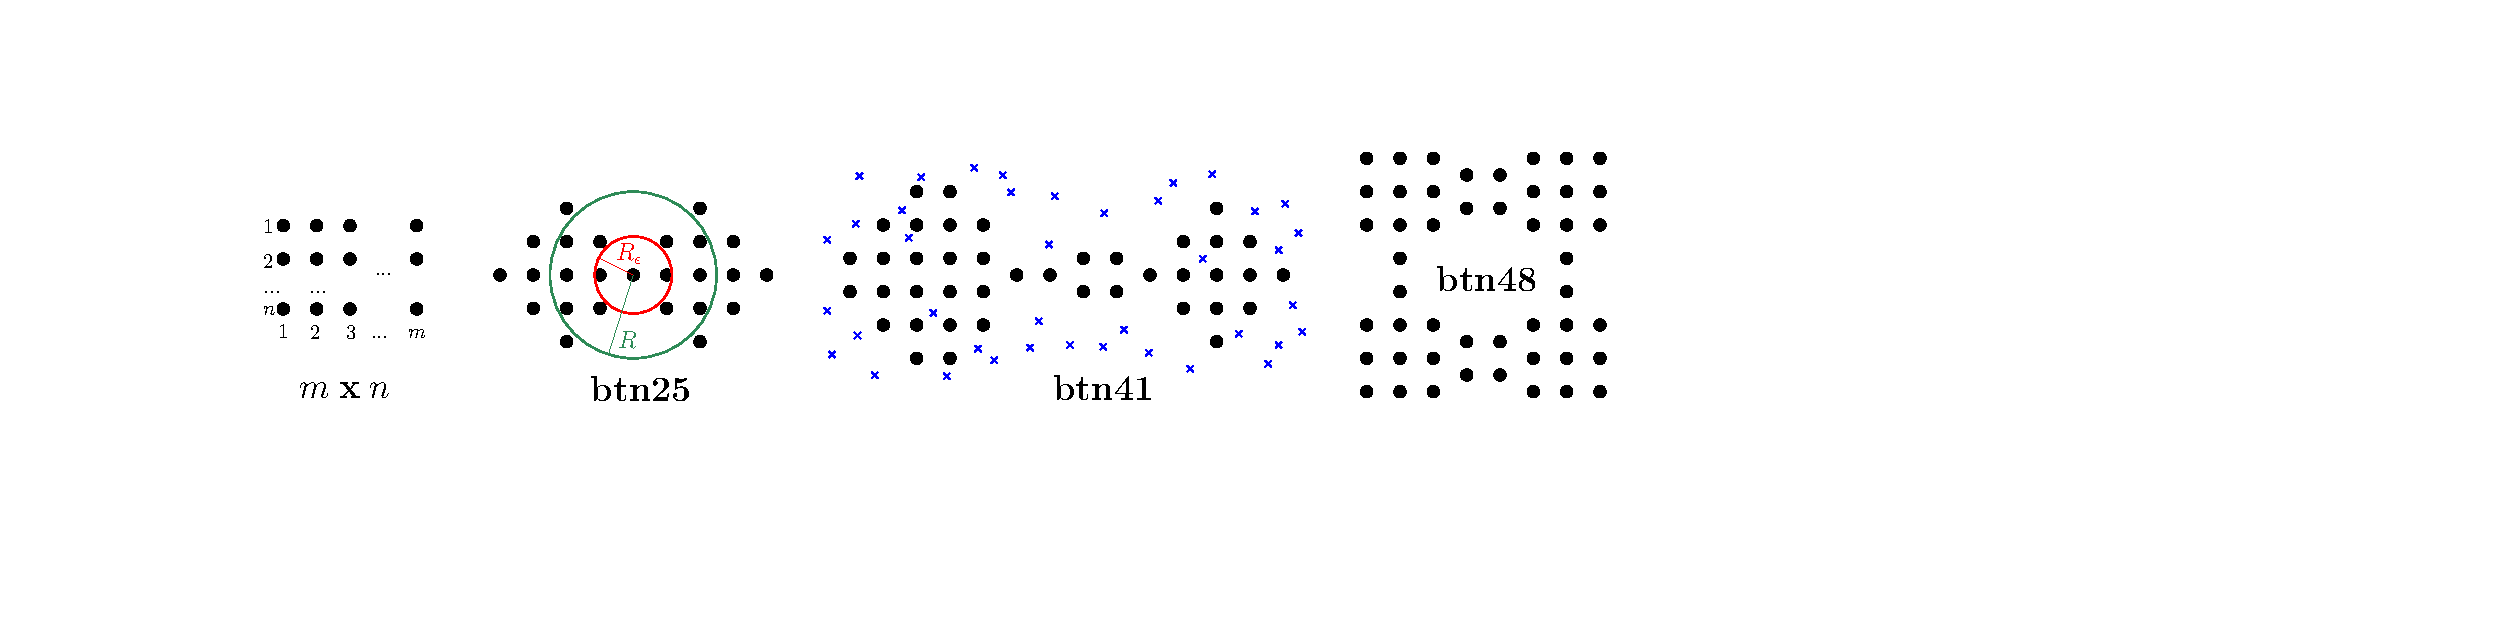
\includegraphics[scale=0.60]{figTopolHorUsersP}
	\end{center}
	\caption{Tipologie di griglie utilizzate.} \label{figP}
\end{figure}
%
Le posizioni degli utenti sono state generate in maniera casuale attorno all'area della griglia, con maggiore probabilità attorno ai bordi (ad esempio, le croci blu in \figurename\ \ref{figP}), assicurandosi che tutti i client si trovassero a distanze minori di $R$ da ciascun punto $i \in P$, per evitare istanze impossibili da risolvere a causa del cattivo posizionamento. \\
Test preliminari per il dimensionamento del dataset hanno dimostrato l'impossibilità di risolvere istanze, con i vincoli temporali e di memoria stabiliti, con un numero di clients $n \geq 30$. \\
Le griglie "complete" impiegate nel dataset, identificate dalla loro dimensione(lunghezza x altezza, in numero di punti) sono le seguenti: 4x8, 6x6, 9x9, 5x10, 6x15, 8x20. Oltre a queste, come già accennato, sono state utilizzate le griglie "speciali" $btn25$, $btn41$, $btn48$.\\
Per ogni griglia e per ogni numero di utenti nell'insieme $\{5, 10, 15, 20, 25, 30\}$ sono state generate 3 istanze casuali, generando in maniera casuale le posizioni degli utenti e le matrici di traffico. \\

\subsection{Relazione tra dimensione delle istanze e tempi di esecuzione}
Nella fase di dimensionamento del dataset abbiamo cercato di identificare quali parametri, di una generica istanza, influissero maggiormente sui tempi di esecuzione di CPLEX, e in che maniera:
\begin{itemize}
	\item Il numero di client influisce notevolmente sulle dimensioni del modello, in quanto da esso dipende direttamente il numero di commodities dell'istanza ($|K| = n(n-1)$), e di conseguenza il numero di variabili $f_{ij}^{sd}$ generate, il numero di vincoli di flusso (\ref{eq:balance}) e il numero di termini dei vincoli (\ref{eq:capTX}) e (\ref{eq:capRX}); 
	\item Il numero di punti della griglia è un altro fattore decisivo per i tempi di esecuzione, poiché la cardinalità dell'insieme di posizioni potenziali $P$ è direttamente proporzionale al numero totale di vincoli generati dal modello;
	\item Il range trasmissivo dei nodi (sia droni che client) influenza la cardinalità dell'insieme di variabili $f_{ij}^{sd}$, in quanto vengono generate solo quelle tali che $d(i,j) \leq R$, e il numero di termini delle sommatorie nei vincoli (\ref{eq:setSub}) e (\ref{eq:setSlb}), in quanto dipendenti dal numero di posizioni potenziali nel range di ciascun nodo. 
\end{itemize} 

\section{Risultati}
Come detto nel \chaptername\ \ref{cap:metodi}, il modello è stato implementato in C++ utilizzando le CPLEX Callable Library (C API), con tempo massimo di esecuzione di 40 minuti, parallelismo deterministico e focus sull'ottimizzazione della memoria. Le istanze sono state risolte su un sistema con 4 processori Intel Xeon E5520 @2.27 GHz e 32 GB di RAM. \\
I risultati ottenuti con questo campione del dataset sono mostrati in \tablename \ref{tabRes}. 
La prima colonna indica il nome della griglia (cioè la sua dimensione, in numero di punti potenziali, in formato lunghezza x altezza) e il numero di utenti, la seconda colonna si riferisce all'elaborazione con CPLEX, e le restanti due alle euristiche. La colonna Time indica il tempo medio delle tre istanze, la colonna Best il miglior tempo registrato, la colonna Drones il numero di droni minimo necessario.  \\
%
\setlength{\tabcolsep}{3.5 pt}
\renewcommand\arraystretch{1.1}
\begin{table} 
	\scriptsize
	\center
	\begin{tabular}{lc|rrr|rrr|rrr}
		\hline
		\multicolumn{2}{c}{\bf Instance} & \multicolumn{3}{|c}{{\bf Cplex 12.6}} & \multicolumn{3}{|c}{{\bf Binary Y}} & \multicolumn{3}{|c}{{\bf Set Y}}\\
		{\bf $P$} & $|V|$ & Time & Best & Drones & Time & Best & Drones & Time & Best & Drones \\
		\hline
		4x8 & 10 & 0.3 & 0.3 & 5 & 0.7 & 0.4 & 4 & 0.2 & 0.1 & 4 \\
		4x8 & 20 & 5.0 & 4.8 & 7 & 9.5 & 7.1 & 8 & 3.6 & 3.4 & 8 \\
		4x8 & 30 & T.L. & T.L. & 32 & T.L & T.L. & 32 & T.L. & T.L. & 32 \\
		6x6 & 10 & 0.42 & 0.4 & 4 & 0.7 & 0.5 & 4 & 0.3 & 0.2 & 4 \\
		6x6 & 20 & 10.3 & 8.9 & 8 & 19.0 & 18.3 & 9 & 8.3 & 7.2 & 8 \\
		6x6 & 30 & T.L. & T.L. & 36 & T.L. & T.L. & 32 & T.L. & T.L. & 32 \\
		9x9 & 10 & 3.25 & 2.8 & 4 & 3.0 & 2.38 & 10 & 3.2 & 2.6 & 4 \\
		9x9 & 20 & T.L. & T.L. & 81 & T.L. & T.L. & 81 & T.L. & T.L. & 81 \\
		9x9 & 30 & T.L. & T.L. & 81 & T.L. & T.L. & 81 & T.L. & T.L. & 81 \\
		btn25 & 10 & 1.03 & 0.9 & 4 & 1.5 & 0.9 & 4 & 0.45 & 0.4 & 4 \\
		btn25 & 20 & 22.5 & 20.8 & 4 & T.L. & T.L. & 25 & T.L. & T.L. & 25 \\
		btn25 & 30 & T.L. & T.L. & 25 & T.L. & T.L. & 25 & T.L. & T.L. & 25 \\
		btn41 & 10 & 7.2 & 4.2 & 4 & 9.2 & 8.3 & 6 & 5.1 & 3.8 & 6 \\
		btn41 & 20 & T.L. & T.L. & 41 & T.L. & T.L. & 3 & T.L. & T.L. & 41 \\
		btn41 & 30 & T.L. & T.L. & 41 & T.L. & T.L. & 3 & T.L. & T.L. & 41 \\
		btn48 & 10 & 1.42 & 1.2 & 4 & 4.1 & 3.9 & 4 & 1.1 & 1.5 & 4 \\
		btn48 & 20 & 32.5 & 30.4 & 4 & T.L. & T.L. & 48 & T.L. & T.L. & 48 \\
		btn48 & 30 & T.L. & T.L. & 48 & T.L. & T.L. & 48 & T.L. & T.L. & 48 \\
		5x10 & 10 & 0.7 & 0.7 & 4 & 1.2 & 0.5 & 5 & 0.8 & 0.5 & 4 \\
		5x10 & 20 & 22.7 & 18.9 & 4 & T.L. & T.L. & 50 & T.L. & T.L. & 50 \\
		5x10 & 30 & T.L. & T.L. & 50 & T.L. & T.L. & 50 & T.L. & T.L. & 50 \\
		6x15 & 10 & 4.6 & 3.3 & 4 & 6.6 & 4.4 & 6 & 5.6 & 4.7 & 6 \\
		6x15 & 20 & T.L. & T.L. & 4 & T.L. & T.L. & 90 & T.L. & T.L. & 90 \\
		6x15 & 30 & T.L. & T.L. & 90 & T.L. & T.L. & 3 & T.L. & T.L. & 90 \\
		\hline
	\end{tabular}
	\normalsize
	\caption{Risultati sperimentali} 
	\label{tabRes}
\end{table}
%

Dai risultati possiamo vedere che mentre l'euristica Binary Y perde praticamente sempre contro i risultati CPLEX, l'euristica Set Y presenta performance estremamente migliori nella maggior parte dei casi. \\ 





 \chapter{Conclusioni} \label{chap:conclusioni}

% **************************** Define Graphics Path **************************
\ifpdf
    \graphicspath{{Chapter8/Figs/Raster/}{Chapter8/Figs/PDF/}{Chapter8/Figs/}}
\else
    \graphicspath{{Chapter8/Figs/Vector/}{Chapter8/Figs/}}
\fi

L'impiego dei droni come strumenti di supporto per scopi civili è in costante crescita, e vengono studiati sempre nuovi metodi di impiego, spinti anche dalle concrete possibilità di business emergenti. \\
L'ambito sperimentale su cui si è concentrata questa tesi è quello di utilizzarli per il deployment rapido e autonomo di una rete di comunicazione di emergenza, da utilizzare in seguito del verificarsi di disastri naturali che hanno compromesso le reti di comunicazione tradizionali.
Per fare ciò i droni vengono equipaggiati con Access Points wireless e posizionati nel range dei client per creare una backbone FANET (Flying Ad-hoc Network), consentendo loro di connettersi e comunicare. \\
In questa tesi abbiamo affrontato lo scenario appena descritto formalizzandolo come un nuovo problema di ottimizzazione combinatoria, l'Interference-aware Drone Ad-hoc Relay Network Configuration problem (I-DARNC). Per il problema, abbiamo proposto una formulazione di programmazione lineare intera mista (Mixed Integer Linear Programming - MILP) capace di posizionare in maniera ottimale il minor numero possibile di droni per raggiungere tutti i client e soddisfare le loro richieste di traffico. Di particolare rilievo è il fatto di aver integrato nel modello una rappresentazione delle problematiche derivanti dai fenomeni di interferenza, che hanno un notevole impatto sulle capacità dei canali wireless utilizzati. A tal fine, abbiamo proposto un modello di interferenza locale e statico per stimare l'impatto della vicinanza reciproca dei droni e/o degli utenti sulla qualità delle comunicazioni. \\
Il modello è stato implementato in C++, utilizzando le librerie di CPLEX, al fine di ottenere con soluzioni off-the-shelf la soluzione ottima del problema. Abbiamo effettuato dei test preliminari per verificare le performance e i limiti del modello, e di fronte all'impossibilità di risolvere istanze medio-grandi in tempi ragionevoli abbiamo sviluppato un algoritmo euristico basata sulla soluzione iterativa di versioni semplificate del modello, ottenute fissando il valore di un opportuno insieme di variabili. \\
Infine abbiamo confrontato le performance degli algoritmi euristici contro quelle di CPLEX su un dataset creato ad-hoc, a causa dell'assenza in letteratura di dataset sufficientemente compatibili con il nostro problema, dimostrando che la complessità intrinseca del problema richieda espressamente l'adozione di algoritmi euristici per istanze di dimensioni realistiche. \\
Possibili sviluppi futuri del lavoro di tesi riguardano la ricerca di formulazioni alternative più efficienti, in termini di riduzione del numero di vincoli e variabili, l'estensione del modello per ridurre il più possibile il set di assunzioni fatte, migliorando così il realismo delle istanze, il perfezionamento del modello di interferenza, per esempio introducendo la presenza di ostacoli naturali e non (vegetazione, montagne, edifici, etc.), e integrandolo in un sistema di validazione per verificare la bontà dei parametri selezionati, iterando fasi di ottimizzazione-validazione, l'introduzione di modelli di random-walk, per simulare il movimento dei client, e di pattern di traffico realistico, l'ampliamento del dataset tramite funzioni di distribuzione dei clients più realistiche, la differenziazione delle caratteristiche di client e droni (diverse capacità e raggi trasmissivi), e lo sviluppo di nuove euristiche, basate su ricerca locale o algoritmi genetici, che risolvano il problema con approcci differenti (per esempio dal punto di vista geometrico dell'intersezione di cerchi, oppure della topologia dei grafi di rete).    



% ********************************** Back Matter *******************************
% Backmatter should be commented out, if you are using appendices after References
%\backmatter

% ********************************** Bibliography ******************************
\begin{spacing}{0.9}

% To use the conventional natbib style referencing
% Bibliography style previews: http://nodonn.tipido.net/bibstyle.php
% Reference styles: http://sites.stat.psu.edu/~surajit/present/bib.htm

\bibliographystyle{ieeetr}
%\bibliographystyle{unsrt} % Use for unsorted references  
%\bibliographystyle{plainnat} % use this to have URLs listed in References
\cleardoublepage
\bibliography{References/references} % Path to your References.bib file


% If you would like to use BibLaTeX for your references, pass `custombib' as
% an option in the document class. The location of 'reference.bib' should be
% specified in the preamble.tex file in the custombib section.
% Comment out the lines related to natbib above and uncomment the following line.

%\printbibliography[heading=bibintoc, title={References}]


\end{spacing}

% ********************************** Appendices ********************************

\begin{appendices} % Using appendices environment for more functunality

%% ******************************* Thesis Appendix A ****************************
\chapter{How to install \LaTeX} 


%% ******************************* Thesis Appendix B ********************************

\chapter{Installing the CUED class file}


\end{appendices}

% *************************************** Index ********************************
\printthesisindex % If index is present

\end{document}
